\documentclass[11pt, letterpaper]{article}

% --- Packages ---
\usepackage[utf8]{inputenc}
\usepackage{geometry}
\usepackage{graphicx}
\usepackage{float}
\usepackage{caption}
% Consolidated hyperref options to forcefully inject metadata
\usepackage[
    hidelinks, 
    hypertexnames=false,
    pdftitle={MapPro and Google My Maps User Guide},
    pdfauthor={Zhun Hao},
    pdfsubject={GNSS Location Measurement and Export Guide}
]{hyperref}
\usepackage{titlesec}
\usepackage{enumitem}
\usepackage{xcolor}
\usepackage{tocloft}
\usepackage{listings}

% --- Page Setup ---
\geometry{top=1in, bottom=1in, left=1in, right=1in}
\raggedbottom

% Hide section numbering but keep them in the Table of Contents
\setcounter{secnumdepth}{0}

% --- Typography & Aesthetics ---
\usepackage{helvet}
\renewcommand{\familydefault}{\sfdefault}
\frenchspacing % Removes the wide, old-fashioned spaces after periods

\definecolor{primary}{RGB}{40, 40, 40}
\definecolor{secondary}{RGB}{100, 100, 100}

% --- Section Formatting ---
\titleformat{\section}{\Large\bfseries\color{primary}}{\thesection}{0em}{}[\titlerule]
\titleformat{\subsection}{\large\bfseries\color{primary}}{\thesubsection}{0em}{}

% --- List Formatting ---
\setlist[itemize]{leftmargin=*, label=\textcolor{secondary}{$\bullet$}, itemsep=0.5em}

% --- Caption Formatting ---
\captionsetup{font=it, textfont=it, justification=centering, margin=1cm, skip=10pt}

% --- TOC Formatting ---
\renewcommand{\cftsecfont}{\large\bfseries\color{primary}} 
\renewcommand{\cftsecpagefont}{\large\bfseries\color{primary}} 
\renewcommand{\cftsecleader}{\cftdotfill{\cftnodots}} 
\setlength{\cftbeforesecskip}{1em} 
\renewcommand{\cftsubsecfont}{\normalsize\color{secondary}} 
\renewcommand{\cftsubsecpagefont}{\normalsize\color{secondary}}

% --- Listings Formatting ---
\lstset{
    basicstyle=\ttfamily\small,
    breaklines=true,
    frame=single,
    backgroundcolor=\color{gray!5},
    rulecolor=\color{gray!30},
    keywordstyle=\color{blue},
    commentstyle=\color{green!50!black},
    stringstyle=\color{orange},
    showstringspaces=false
}

% --- Begin Document ---
\begin{document}

% =========================================================
% TITLE PAGE
% =========================================================
\begin{titlepage}
    \centering
    \vspace*{2in}
    
    {\Huge\bfseries\color{primary} MapPro GNSS Survey \\[0.5ex] \& Google My Maps Guide\par}
    
    \vspace{1.5in}
    
    {\Large\color{secondary} A comprehensive guide for location measurement using the MapPro companion software on S60 devices, followed by coordinate translation and importing to Google My Maps.\par}
    
    \vfill
    
    % Automatically inserts today's date
    {\large \today\par}
\end{titlepage}

% =========================================================
% TABLE OF CONTENTS
% =========================================================
\tableofcontents
\clearpage

% =========================================================
\section{Overview \& System Prerequisites}
% =========================================================

This guide describes the workflow for using the companion \textbf{MapPro} survey application on an \textbf{S60} mobile device to capture high-accuracy GNSS location measurements, export the survey data in CSV format, and upload the points to \textbf{Google My Maps} for visualization.

\subsection{Coordinate Formatting Issue}
The S60 GNSS receiver records and exports latitude and longitude coordinates as packed Degrees-Minutes-Seconds (DMS) format with raw byte separators (specifically incorporating \texttt{0xB0} degree signs and \texttt{0x1A} minute/second marks), such as:
\begin{center}
    \texttt{N 1° 21' 11.2189"} \quad $\rightarrow$ \quad bytes: \quad \texttt{N1[0xB0]21[0x1A]11.2189[0x1A]}
\end{center}
Because Google My Maps only supports standard decimal degrees (e.g. \texttt{1.353116}), importing the raw exported CSV directly will fail. To resolve this, a companion Python post-processing script, \texttt{csv\_to\_mymaps.py}, must be run on the exported CSV before importing. This script:
\begin{itemize}
    \item Parses the packed DMS angles into standard decimal degrees using high-precision Decimal math.
    \item Safely strips XML-illegal control bytes (e.g. \texttt{0x1A}) that would otherwise corrupt exported KMLs or cause GIS tools to reject the files.
    \item Sanitizes non-numeric fields against spreadsheet formula injection.
\end{itemize}

\subsection{Google My Maps Limitations}
Keep in mind the following platform constraints when planning your survey:
\begin{itemize}
    \item Maximum of \textbf{2,000 rows} per layer.
    \item Maximum of \textbf{10 layers} per map.
    \item Maximum file size of \textbf{5 MB} per layer.
    \item Maximum of \textbf{100 photos} per import.
\end{itemize}

\clearpage

% =========================================================
\section{Step-by-Step GNSS Survey Procedure}
% =========================================================

\subsection{Step 1: Launch MapPro}
Locate and tap the \textbf{Map Pro} application icon in the S60 device's application drawer to launch the software.

\begin{figure}[H]
    \centering
    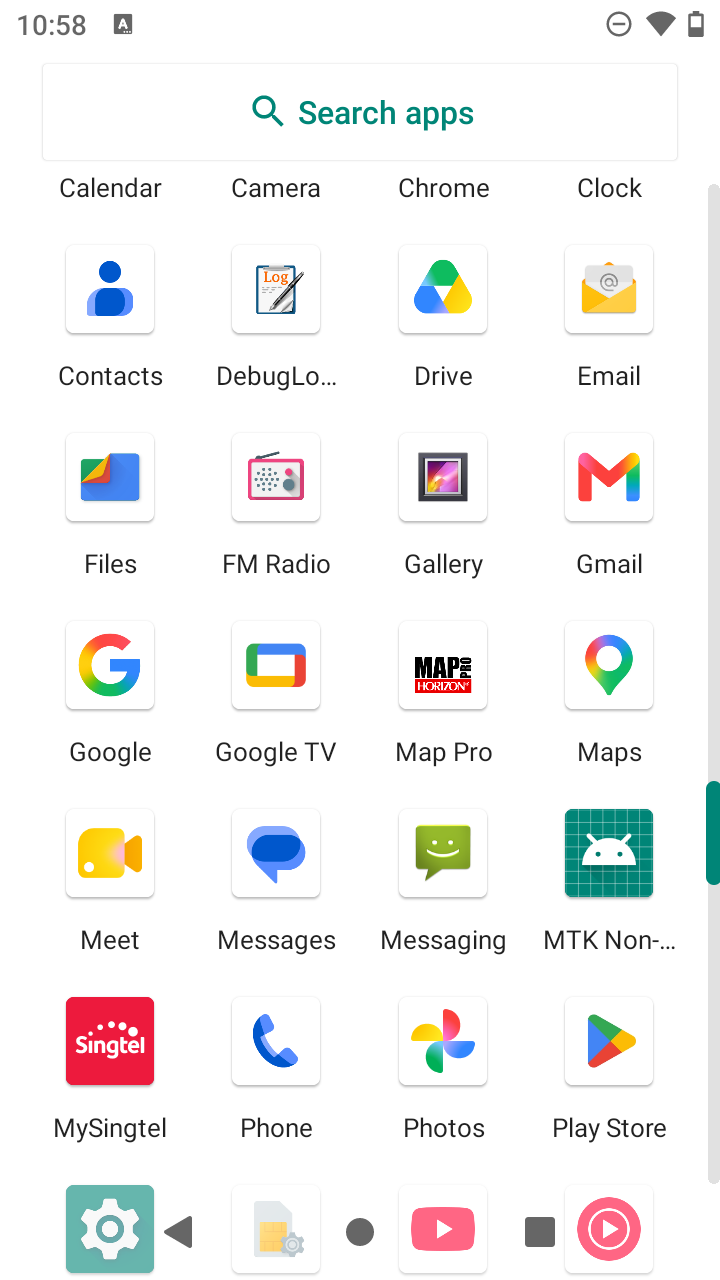
\includegraphics[width=0.45\textwidth]{images/step_1_open_map_pro.png}
    \caption*{Application drawer showing the Map Pro application launcher.}
\end{figure}

\subsection{Step 2: Access Project Manager}
From the default MapPro screen, ensure the \textbf{Project} tab at the bottom is selected. Select the \textbf{Project Manager} menu item at the top of the list.

\begin{figure}[H]
    \centering
    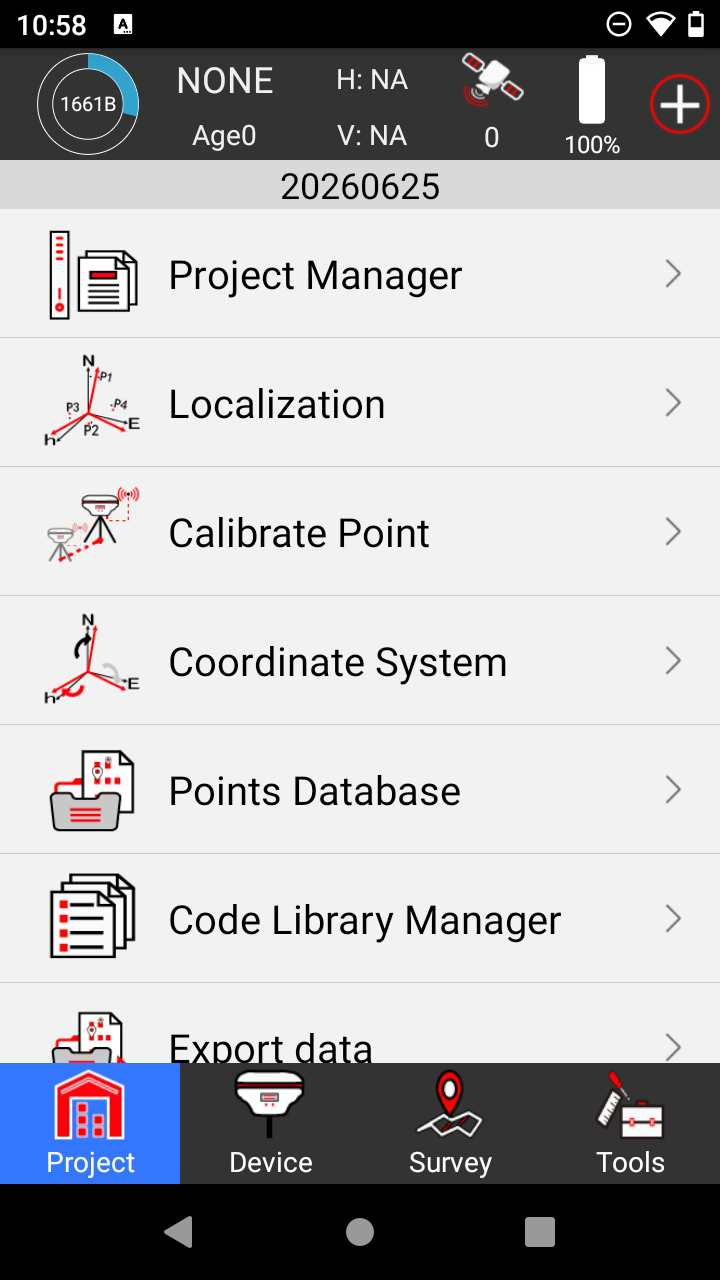
\includegraphics[width=0.45\textwidth]{images/step_2_mappro_screen_open_project_manager.png}
    \caption*{Project tab showing Project Manager, Localization, and other settings.}
\end{figure}

\clearpage

\subsection{Step 3: Create a New Project}
In the Project Manager window, click the \textbf{New} button located in the bottom-left corner to initiate a new project.

\begin{figure}[H]
    \centering
    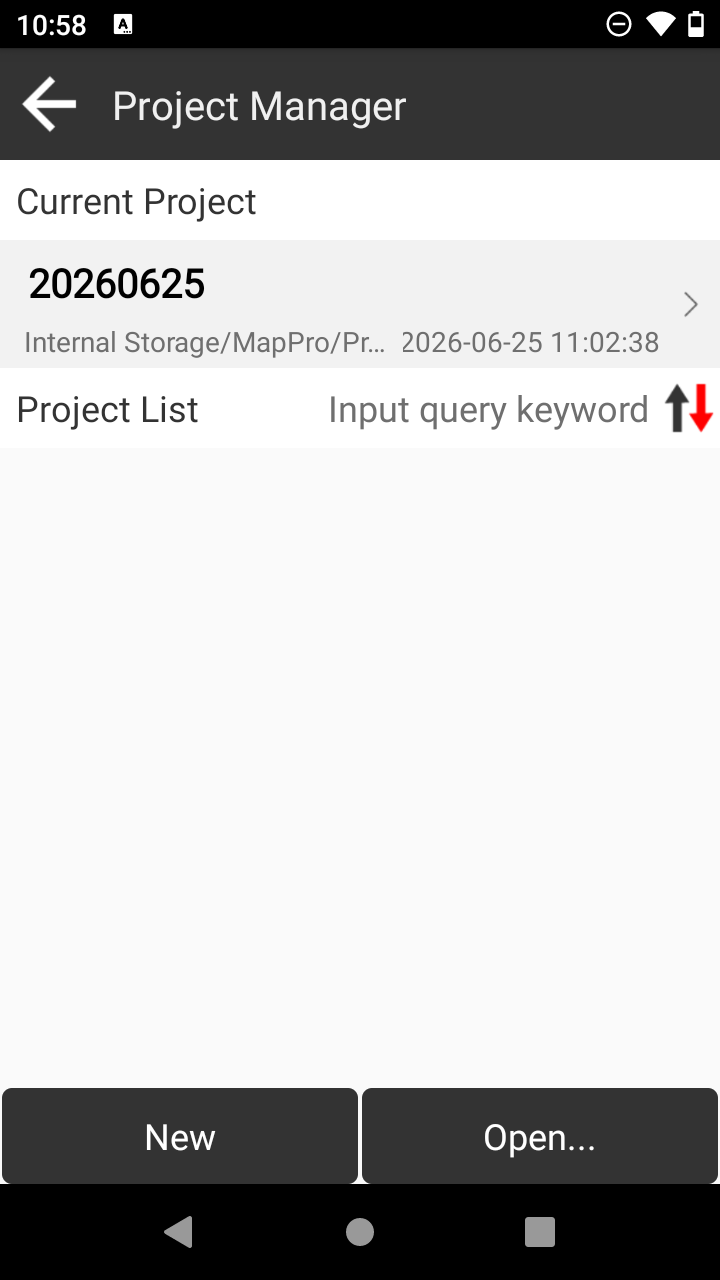
\includegraphics[width=0.45\textwidth]{images/step_3_create_a_new_project.png}
    \caption*{Project Manager listing current active project and available options.}
\end{figure}

\subsection{Step 4: Configure Project Details}
Enter your project details on the Create Project screen. The \textbf{Project Name} will default to the current date (e.g., \texttt{20260626}). Confirm the storage path is correct and click \textbf{Next}.

\begin{figure}[H]
    \centering
    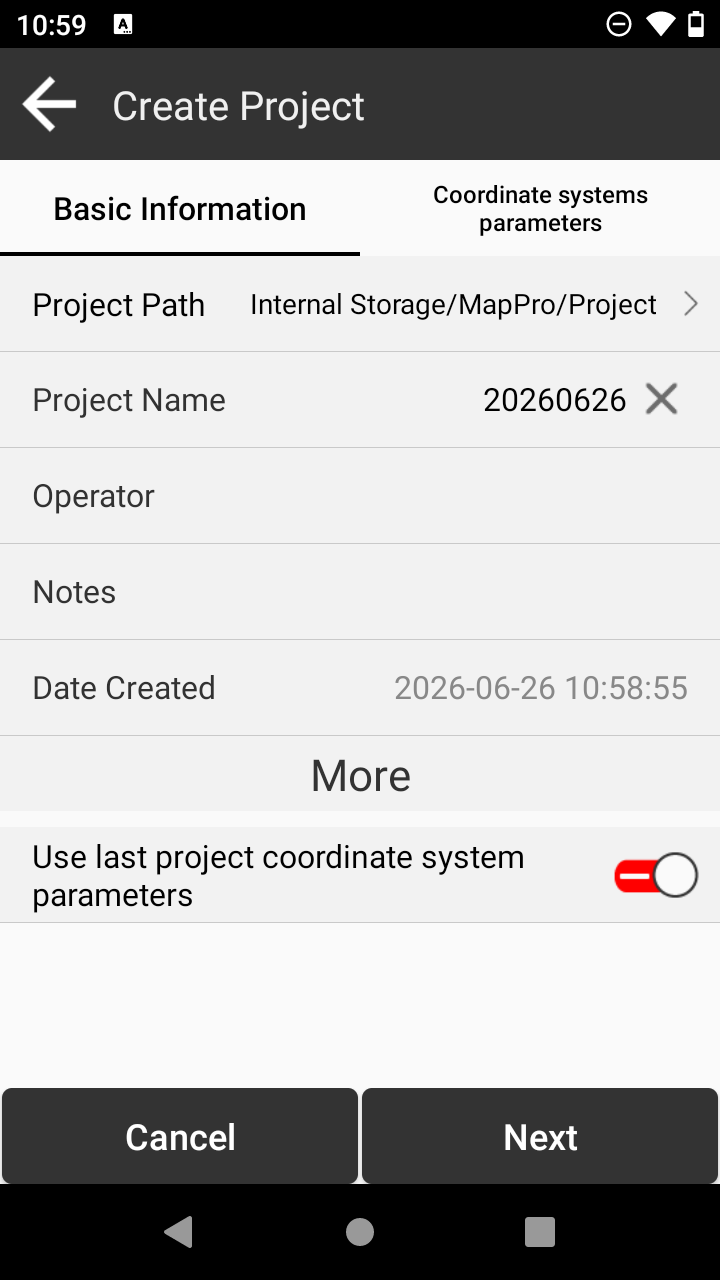
\includegraphics[width=0.45\textwidth]{images/step_4_keep_default_value_next.png}
    \caption*{Setting the basic project details and directories.}
\end{figure}

\clearpage

\subsection{Step 5: Confirm Coordinate System Parameters}
Confirm the coordinate system settings. The Ellipsoid Parameter should default to \textbf{WGS84} and the Projections Parameter to \textbf{Transverse Mercator}. Click \textbf{OK} to finalize project creation.

\begin{figure}[H]
    \centering
    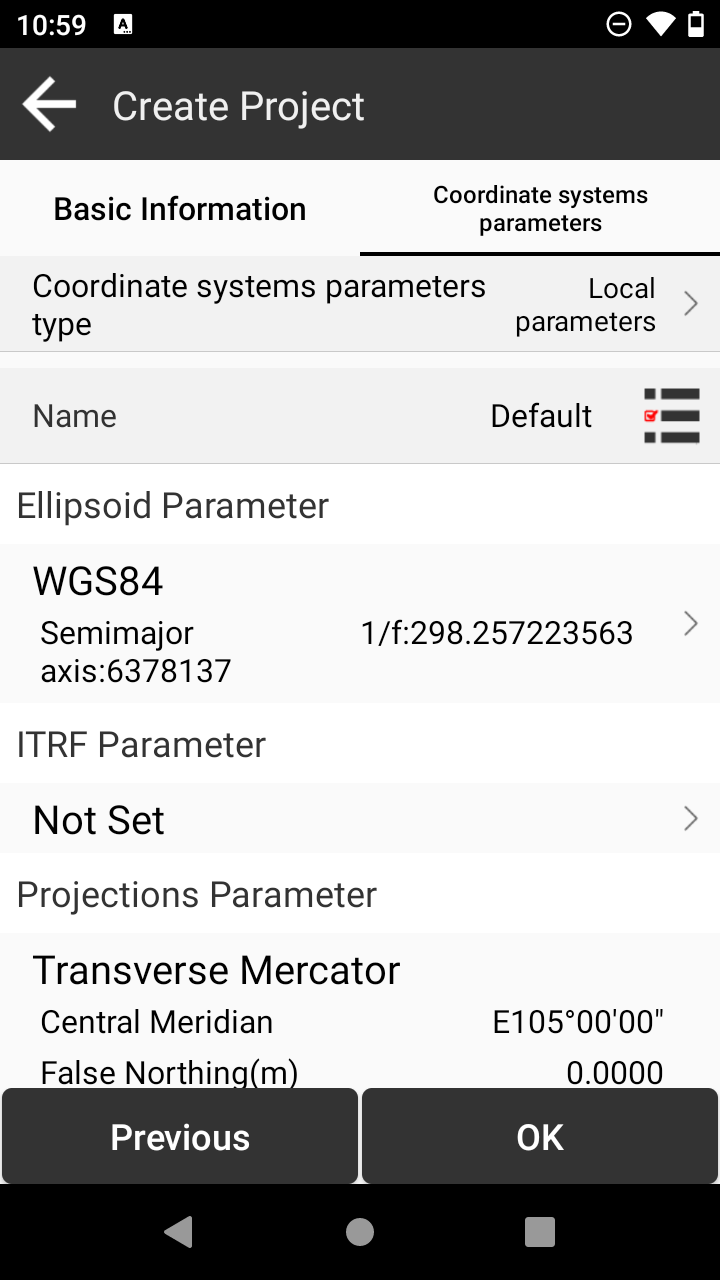
\includegraphics[width=0.45\textwidth]{images/step_5_ok.png}
    \caption*{Coordinate system configurations showing ellipsoidal parameters.}
\end{figure}

\subsection{Step 6: Go to Survey Mode}
Tap the \textbf{Survey} tab at the bottom of the screen, and select the \textbf{Point Survey} option from the menu list.

\begin{figure}[H]
    \centering
    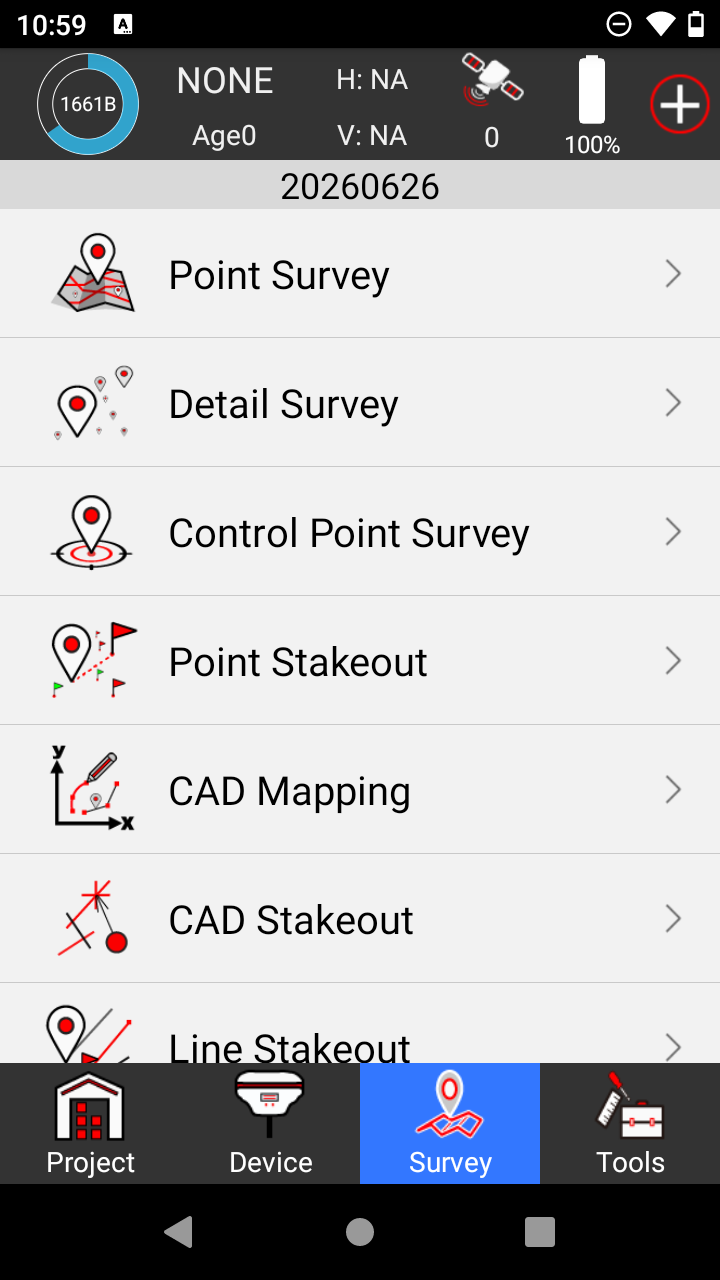
\includegraphics[width=0.45\textwidth]{images/step_7_go_survey_and_select_point_survey.png}
    \caption*{Survey options tab showcasing the Point Survey selection.}
\end{figure}

\clearpage

\subsection{Step 7: Calibrate GNSS Receiver \& Verify Fixed Status}
Upon entering the Point Survey screen, check the status indicator in the top-left corner. If it displays \textbf{FIXED} in green, the receiver is calibrated and ready. If it requires IMU/tilt calibration, shake the S60 device in a figure-eight pattern until the status indicator turns green.

\begin{figure}[H]
    \centering
    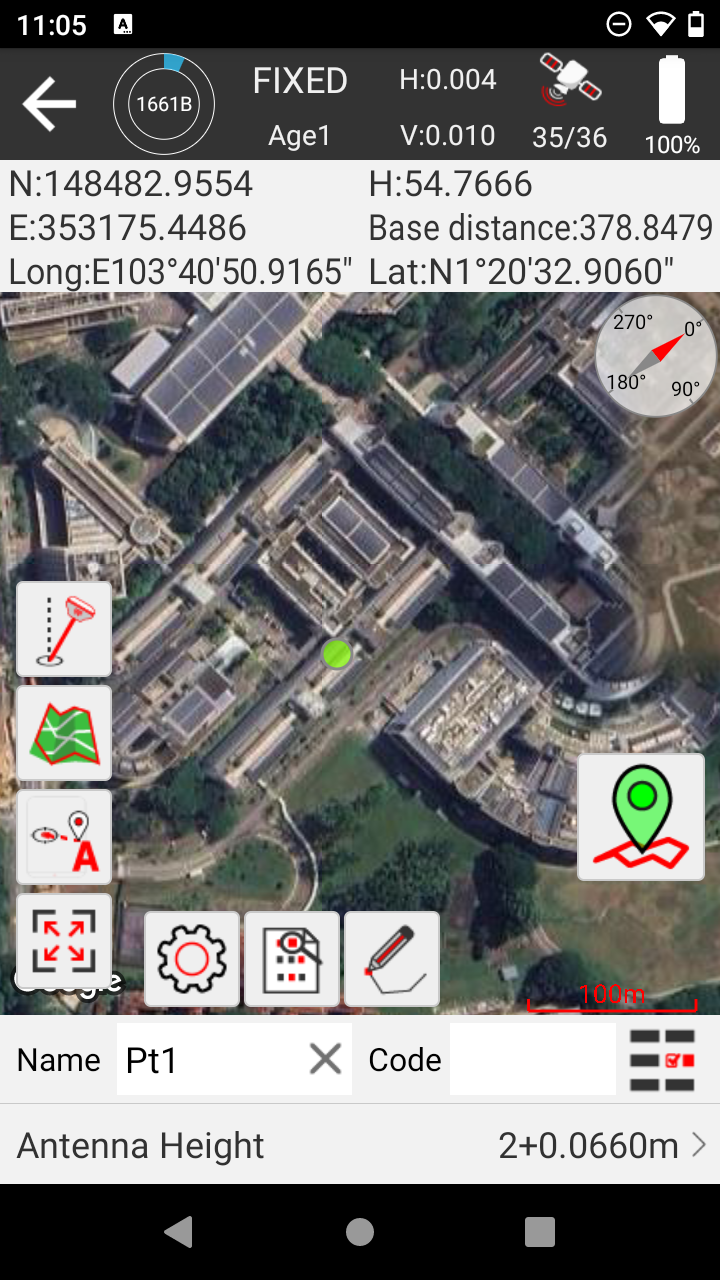
\includegraphics[width=0.45\textwidth]{images/step_6_you_can_start_measurment_straight_away_if_green_calbarte_by_shaking_.png}
    \caption*{Main survey screen showing a FIXED satellite solution and position readout.}
\end{figure}

\subsection{Step 8: Collect Point Measurement}
In the Point Survey panel, configure the point \textbf{Name} (e.g., \texttt{Pt1}), \textbf{Antenna Height} (e.g., \texttt{2+0.0660m}), and \textbf{Code}. Start the measurement. The application will show a dialog counting down the captured epochs (e.g., \texttt{Collecting <4/5>}) to average the position.

\begin{figure}[H]
    \centering
    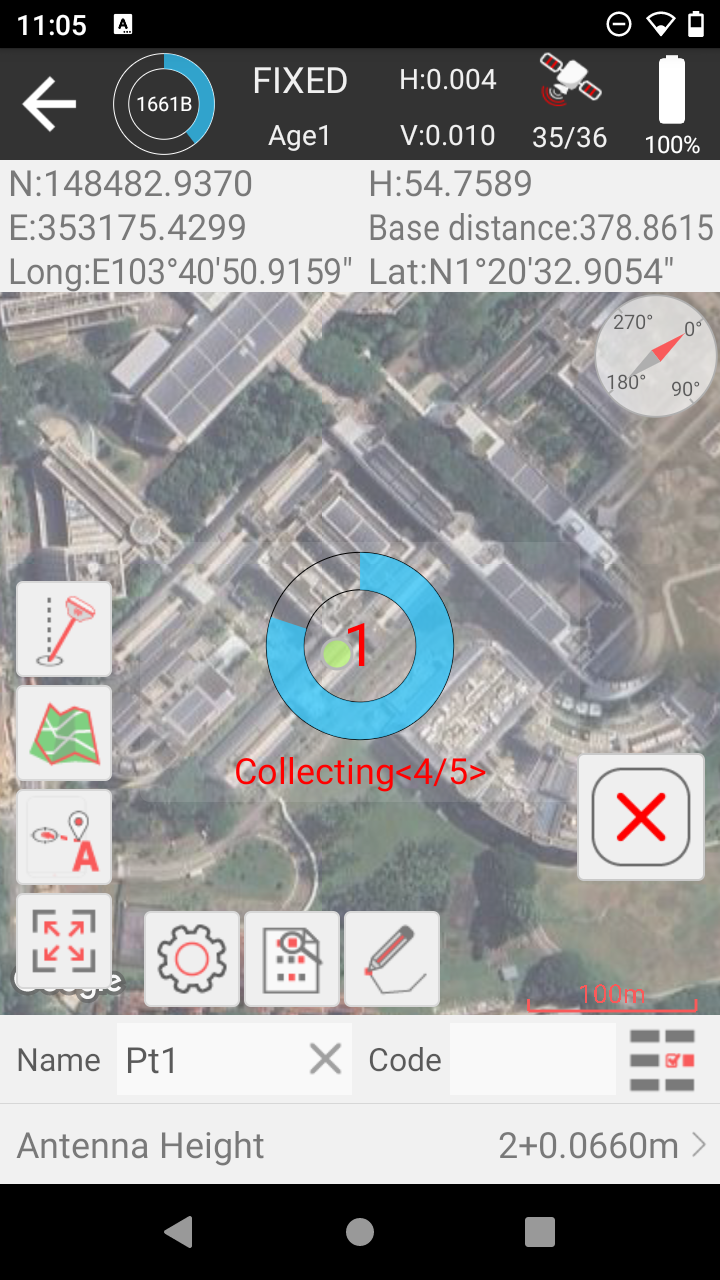
\includegraphics[width=0.45\textwidth]{images/step_8.png}
    \caption*{The active point collection process averaging multiple epochs.}
\end{figure}

\clearpage

\subsection{Step 9: Collect Subsequent Points}
Return to the Point Survey screen and continue measuring subsequent locations (e.g., \texttt{Pt2}). Verify that the receiver status remains \textbf{FIXED} in green and the antenna height is correct before initiating each collection.

\begin{figure}[H]
    \centering
    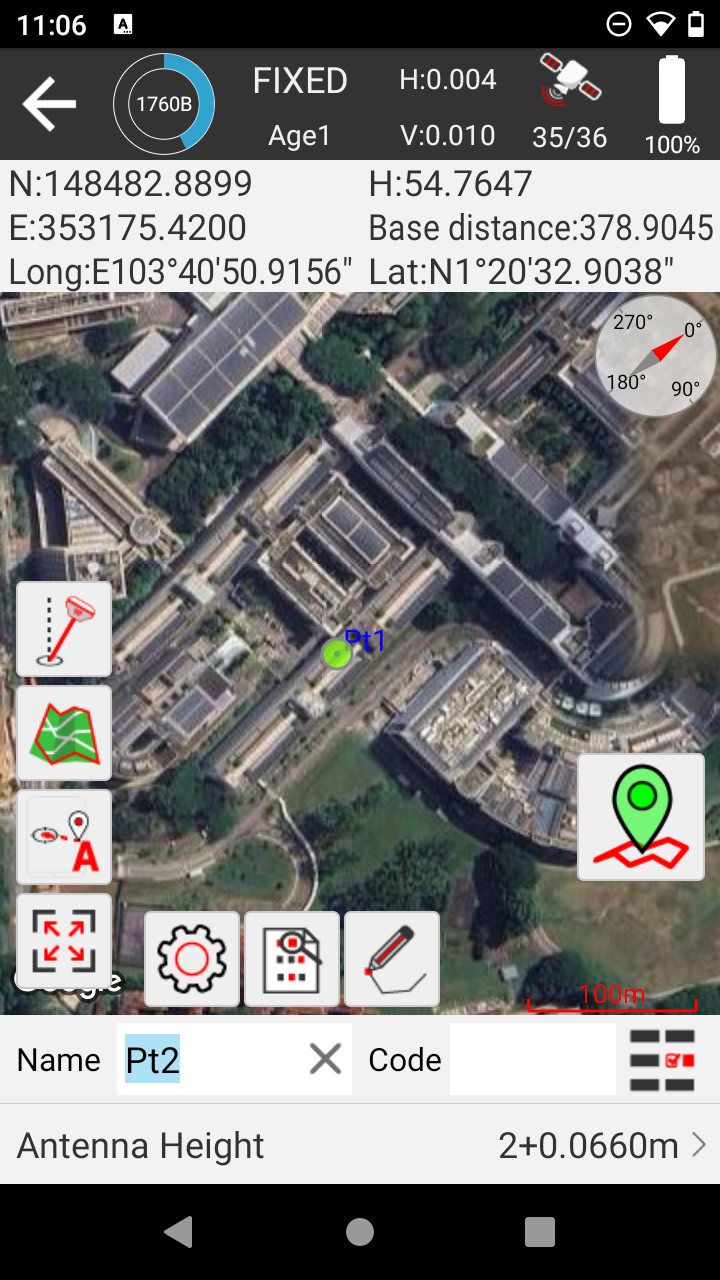
\includegraphics[width=0.45\textwidth]{images/step_10.png}
    \caption*{Measuring subsequent point Pt2 with active satellite solutions.}
\end{figure}

\clearpage

% =========================================================
% DATA EXPORTING
% =========================================================
\section{Data Exporting}

\subsection{Step 10: Open Points Database}
To view and verify your recorded survey points, open the \textbf{Points Database} (located under either the Project or Tools menu). You can view detailed information for each point (e.g., \texttt{Pt1}) including coordinate readings, elevation, and timestamp. Tapping the \textbf{Export} button at the bottom right of this screen will launch the export workflow.

\begin{figure}[H]
    \centering
    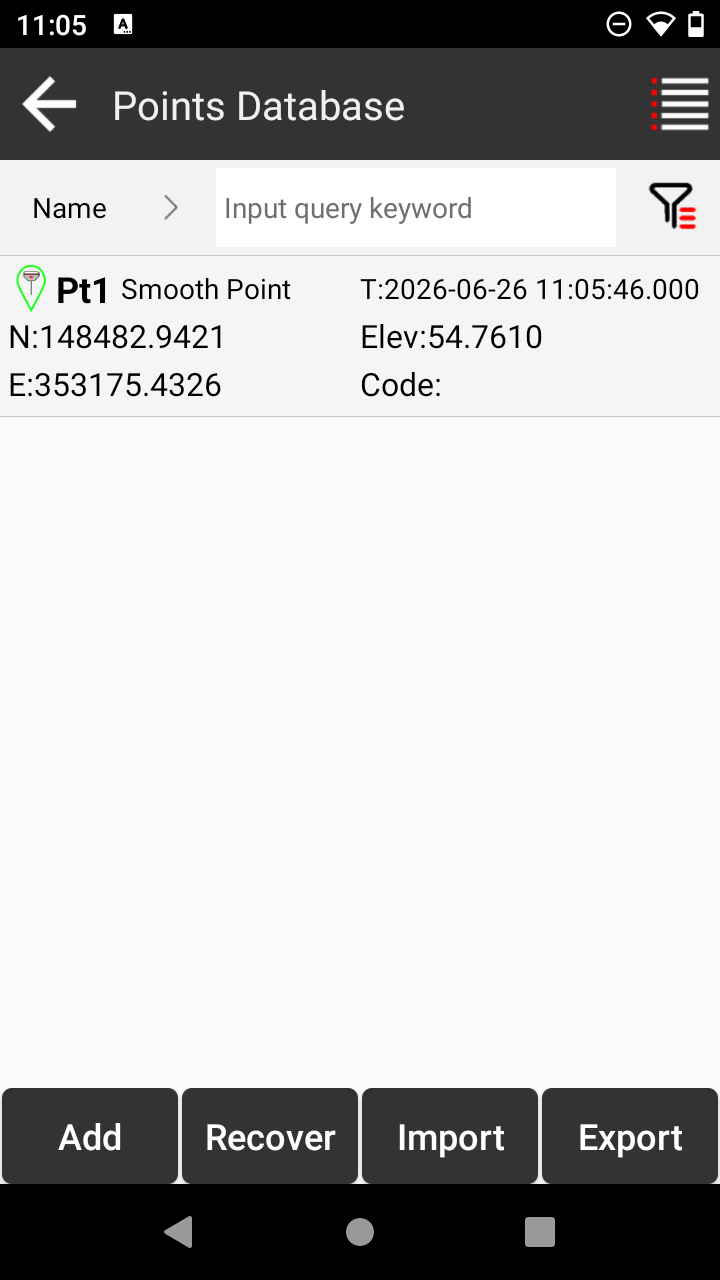
\includegraphics[width=0.45\textwidth]{images/step_9.png}
    \caption*{Points Database containing the measured "Smooth Point" details and the Export function.}
\end{figure}

\subsection{Step 11: Alternative Access from Project Menu}
Alternatively, you can access the export workflow by navigating back to the \textbf{Project} tab at the bottom of the screen and selecting \textbf{Export data} from the list.

\begin{figure}[H]
    \centering
    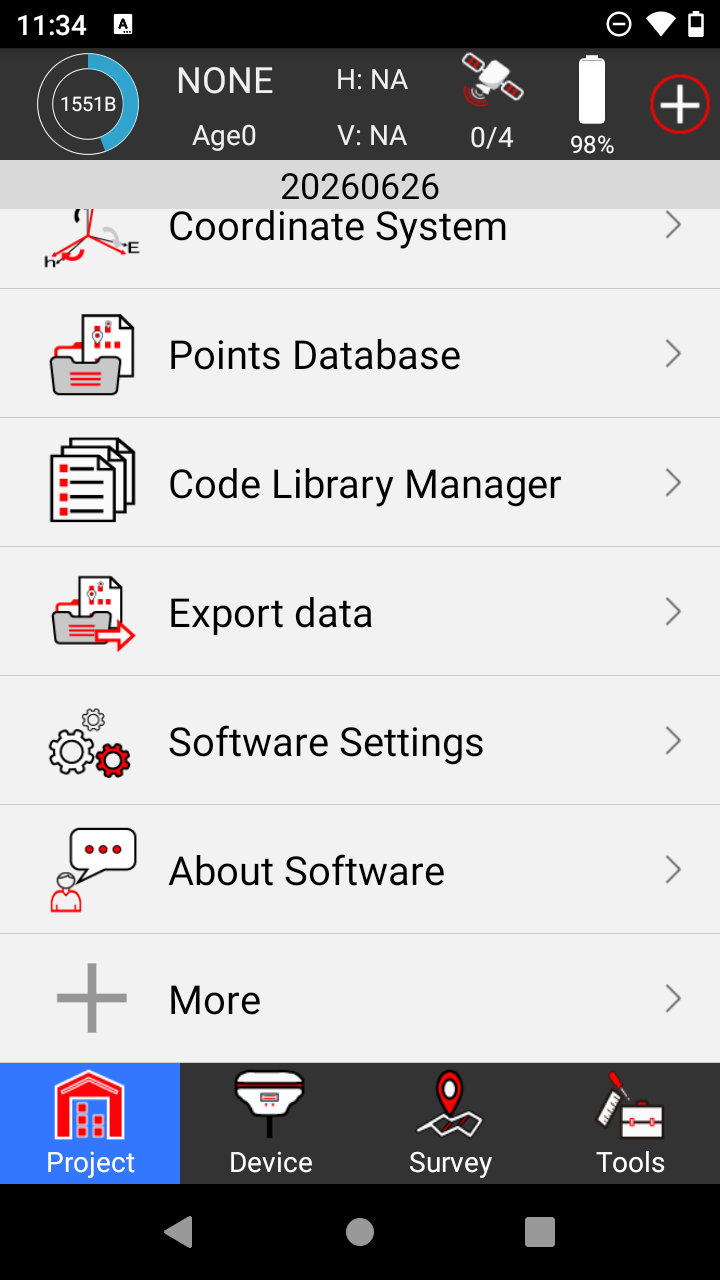
\includegraphics[width=0.45\textwidth]{images/step_11.png}
    \caption*{Selecting the Export data utility from the Project tab.}
\end{figure}

\clearpage

\subsection{Step 12: Open File Format Options}
The export screen displays the default output path (\texttt{Internal Storage/MapPro/Export}) and the file name (which defaults to the project name). Tap on the \textbf{Choose Export File Format} selector.

\begin{figure}[H]
    \centering
    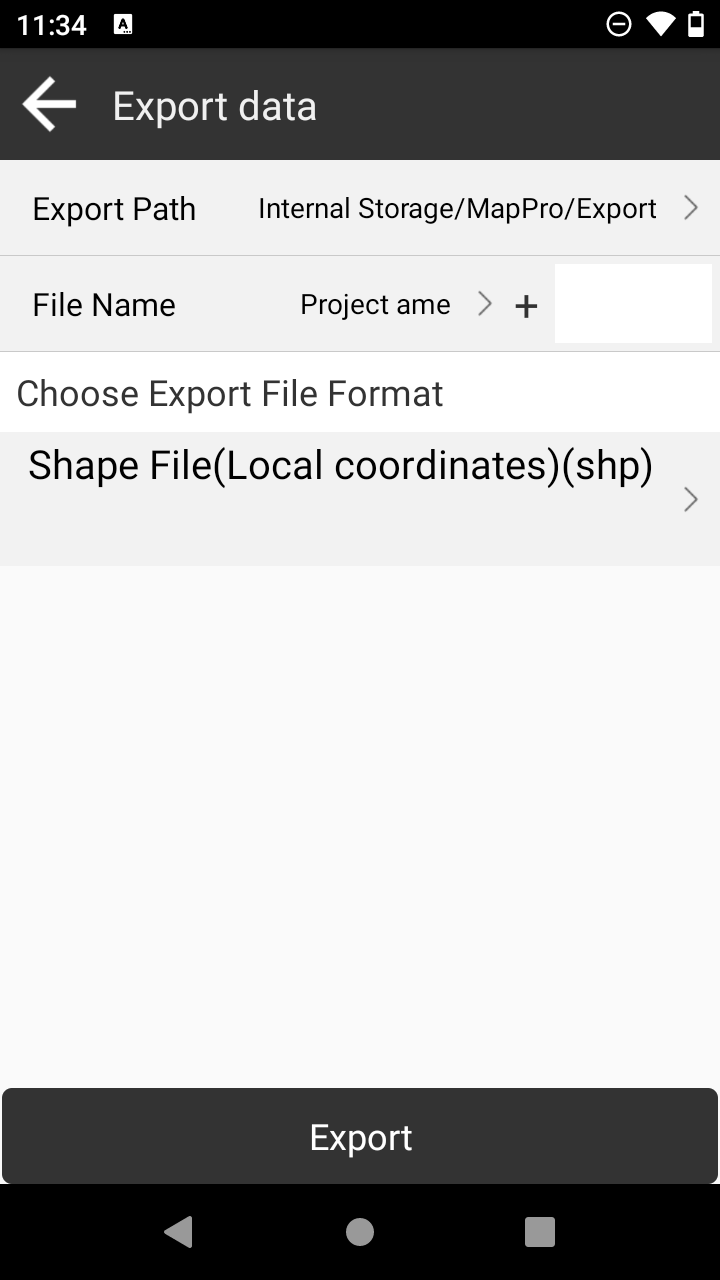
\includegraphics[width=0.45\textwidth]{images/step_12.png}
    \caption*{Initial export data screen displaying the storage directory.}
\end{figure}

\subsection{Step 13: Select CSV Survey Point Format}
In the file format pop-up, scroll and select \textbf{Survey point data format(csv)}. This format contains the required \texttt{Latitude} and \texttt{Longitude} columns necessary for mapping. Click \textbf{OK}.

\begin{figure}[H]
    \centering
    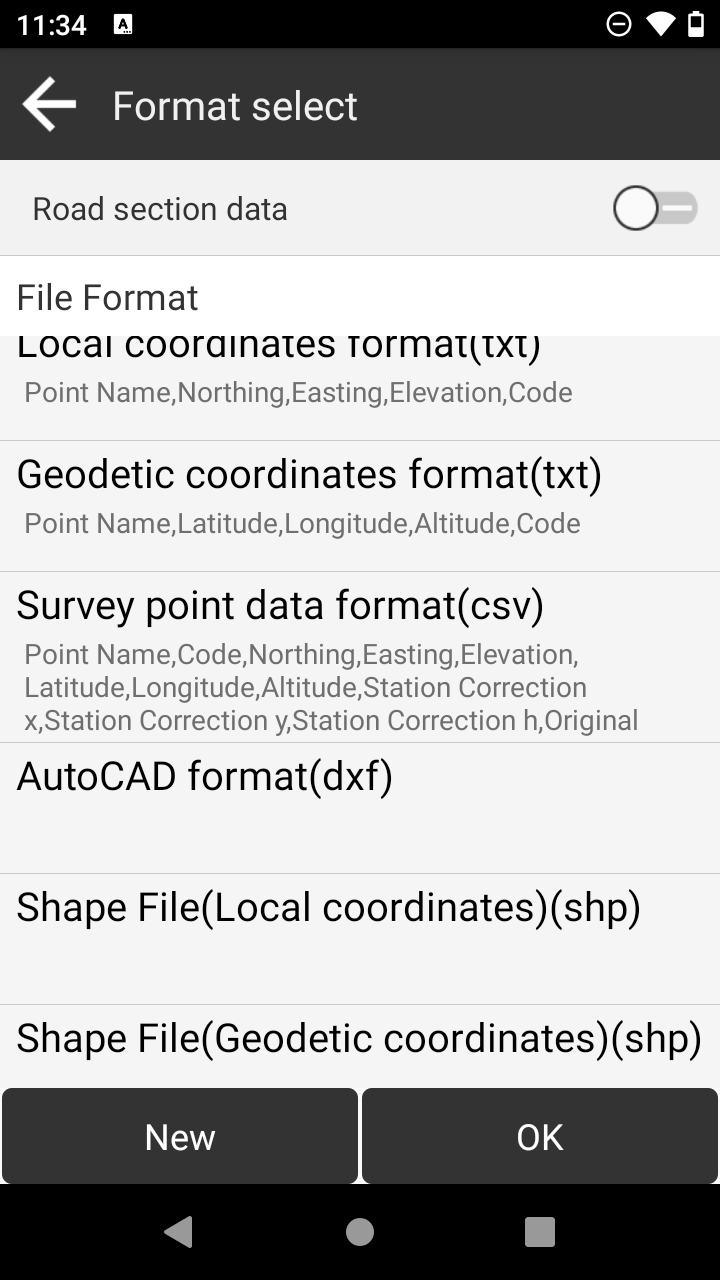
\includegraphics[width=0.45\textwidth]{images/step_13.png}
    \caption*{Selecting the Survey point data format (csv) option from the popup.}
\end{figure}

\clearpage

\subsection{Step 14: Configure Units and Export}
Back on the Export page, confirm the \textbf{Distance Unit} is set to \textbf{Meter} and the \textbf{Angle format} is set to \textbf{dd°mm'ss.ssss"}. Click the \textbf{Export} button at the bottom of the screen.

\begin{figure}[H]
    \centering
    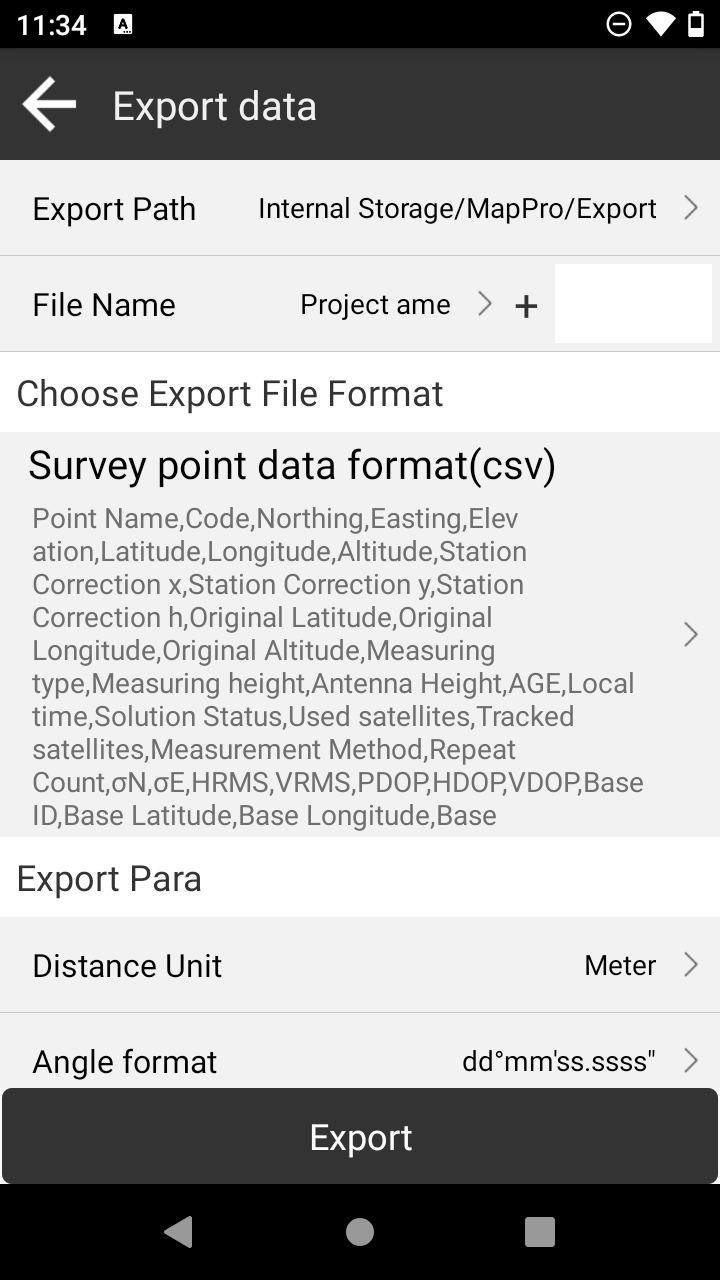
\includegraphics[width=0.45\textwidth]{images/step_14.png}
    \caption*{Configuring final angle formats and units before exporting.}
\end{figure}

\subsection{Step 15: Share Exported File}
A prompt will appear stating "The file was exported successfully, do you want to share it?". Click \textbf{Yes} to transfer the file via your preferred method (email, Bluetooth, or messaging application) to your computer, or click \textbf{No} to retrieve it manually via USB from the \texttt{Internal Storage/MapPro/Export} folder.

\begin{figure}[H]
    \centering
    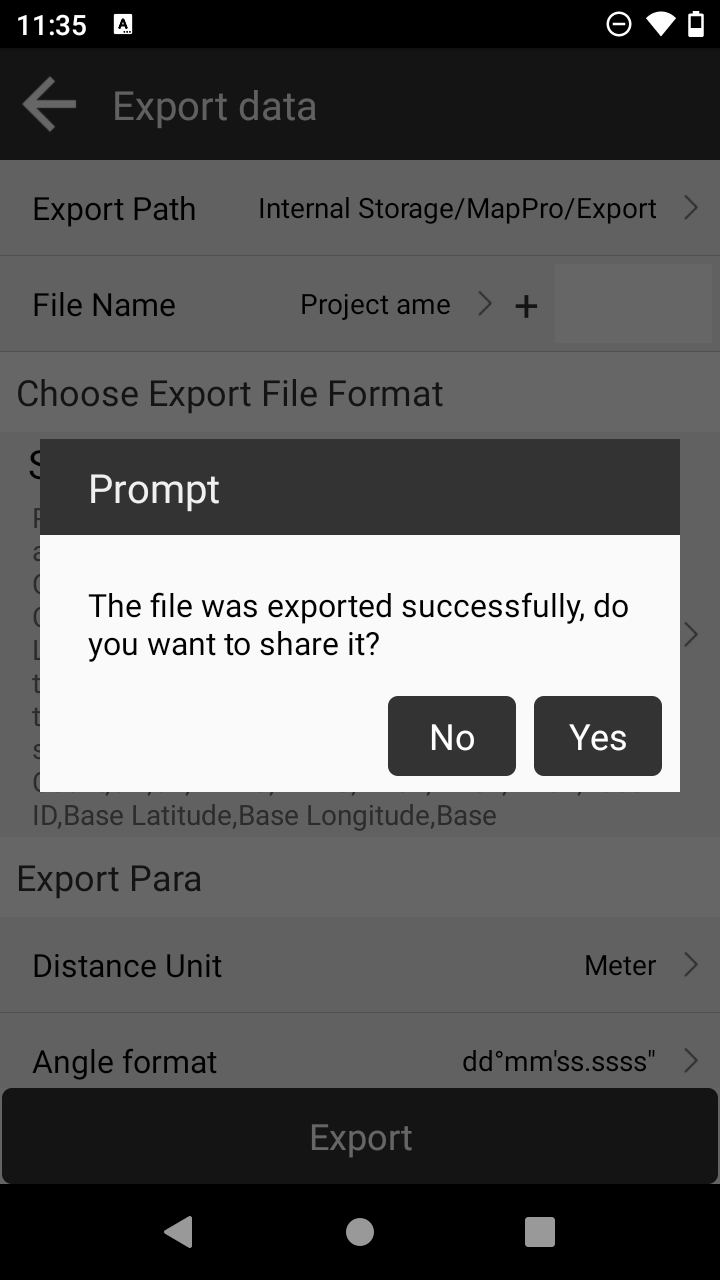
\includegraphics[width=0.45\textwidth]{images/step_15.png}
    \caption*{Successful file export and sharing dialog.}
\end{figure}

\clearpage

% =========================================================
\section{File Transfer to Laptop via OpenMTP}
% =========================================================

\subsection{Step 16: Connect Device and Open MapPro Folder in OpenMTP}
Connect the S60 device to your laptop using a USB data cable. Ensure that the USB connection mode on the S60 is set to **MTP (File Transfer)**. On your laptop, launch the **OpenMTP** application. In OpenMTP's device tab panel displaying the S60 internal shared storage (\texttt{SD55}), locate and double-click the \textbf{MapPro} folder.

\begin{figure}[H]
    \centering
    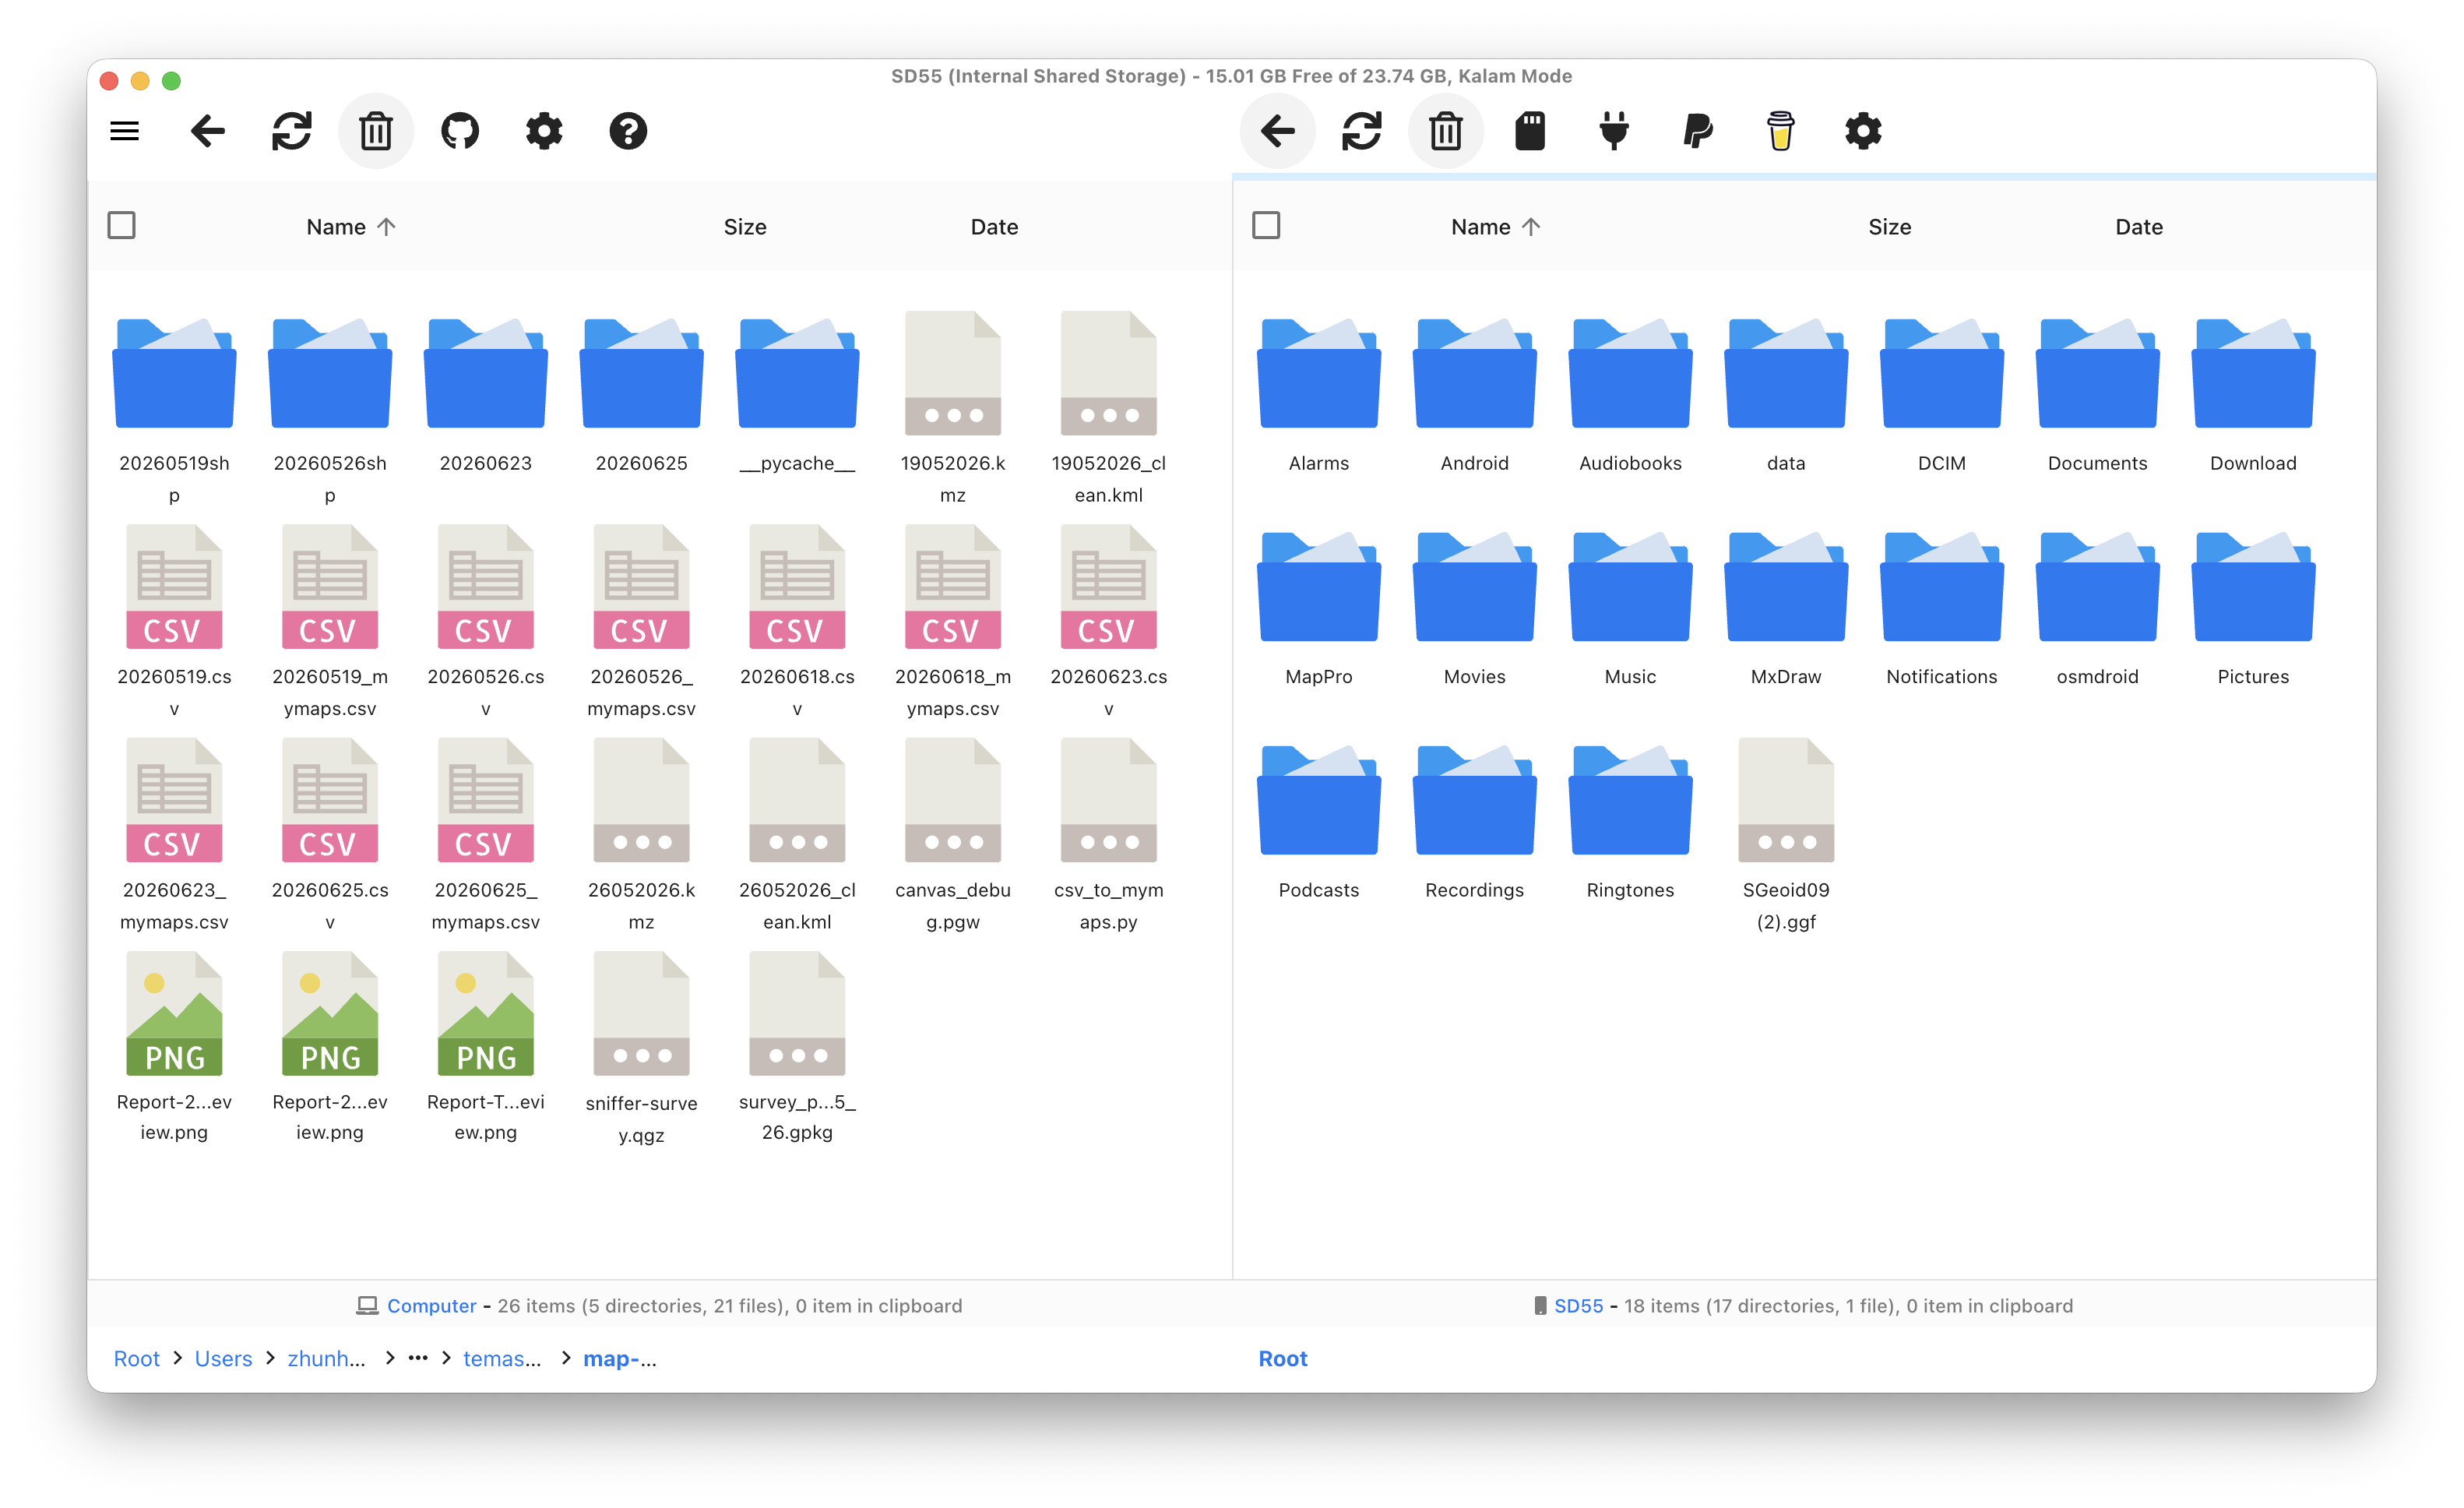
\includegraphics[width=0.85\textwidth]{images/open_mtp_1_go_to_mappro.png}
    \caption*{Accessing the internal storage of the S60 device inside OpenMTP and locating the MapPro directory.}
\end{figure}

\subsection{Step 17: Navigate to the Export Folder}
Inside the MapPro directory in OpenMTP, locate and double-click the \textbf{Export} folder to access all exported data files.

\begin{figure}[H]
    \centering
    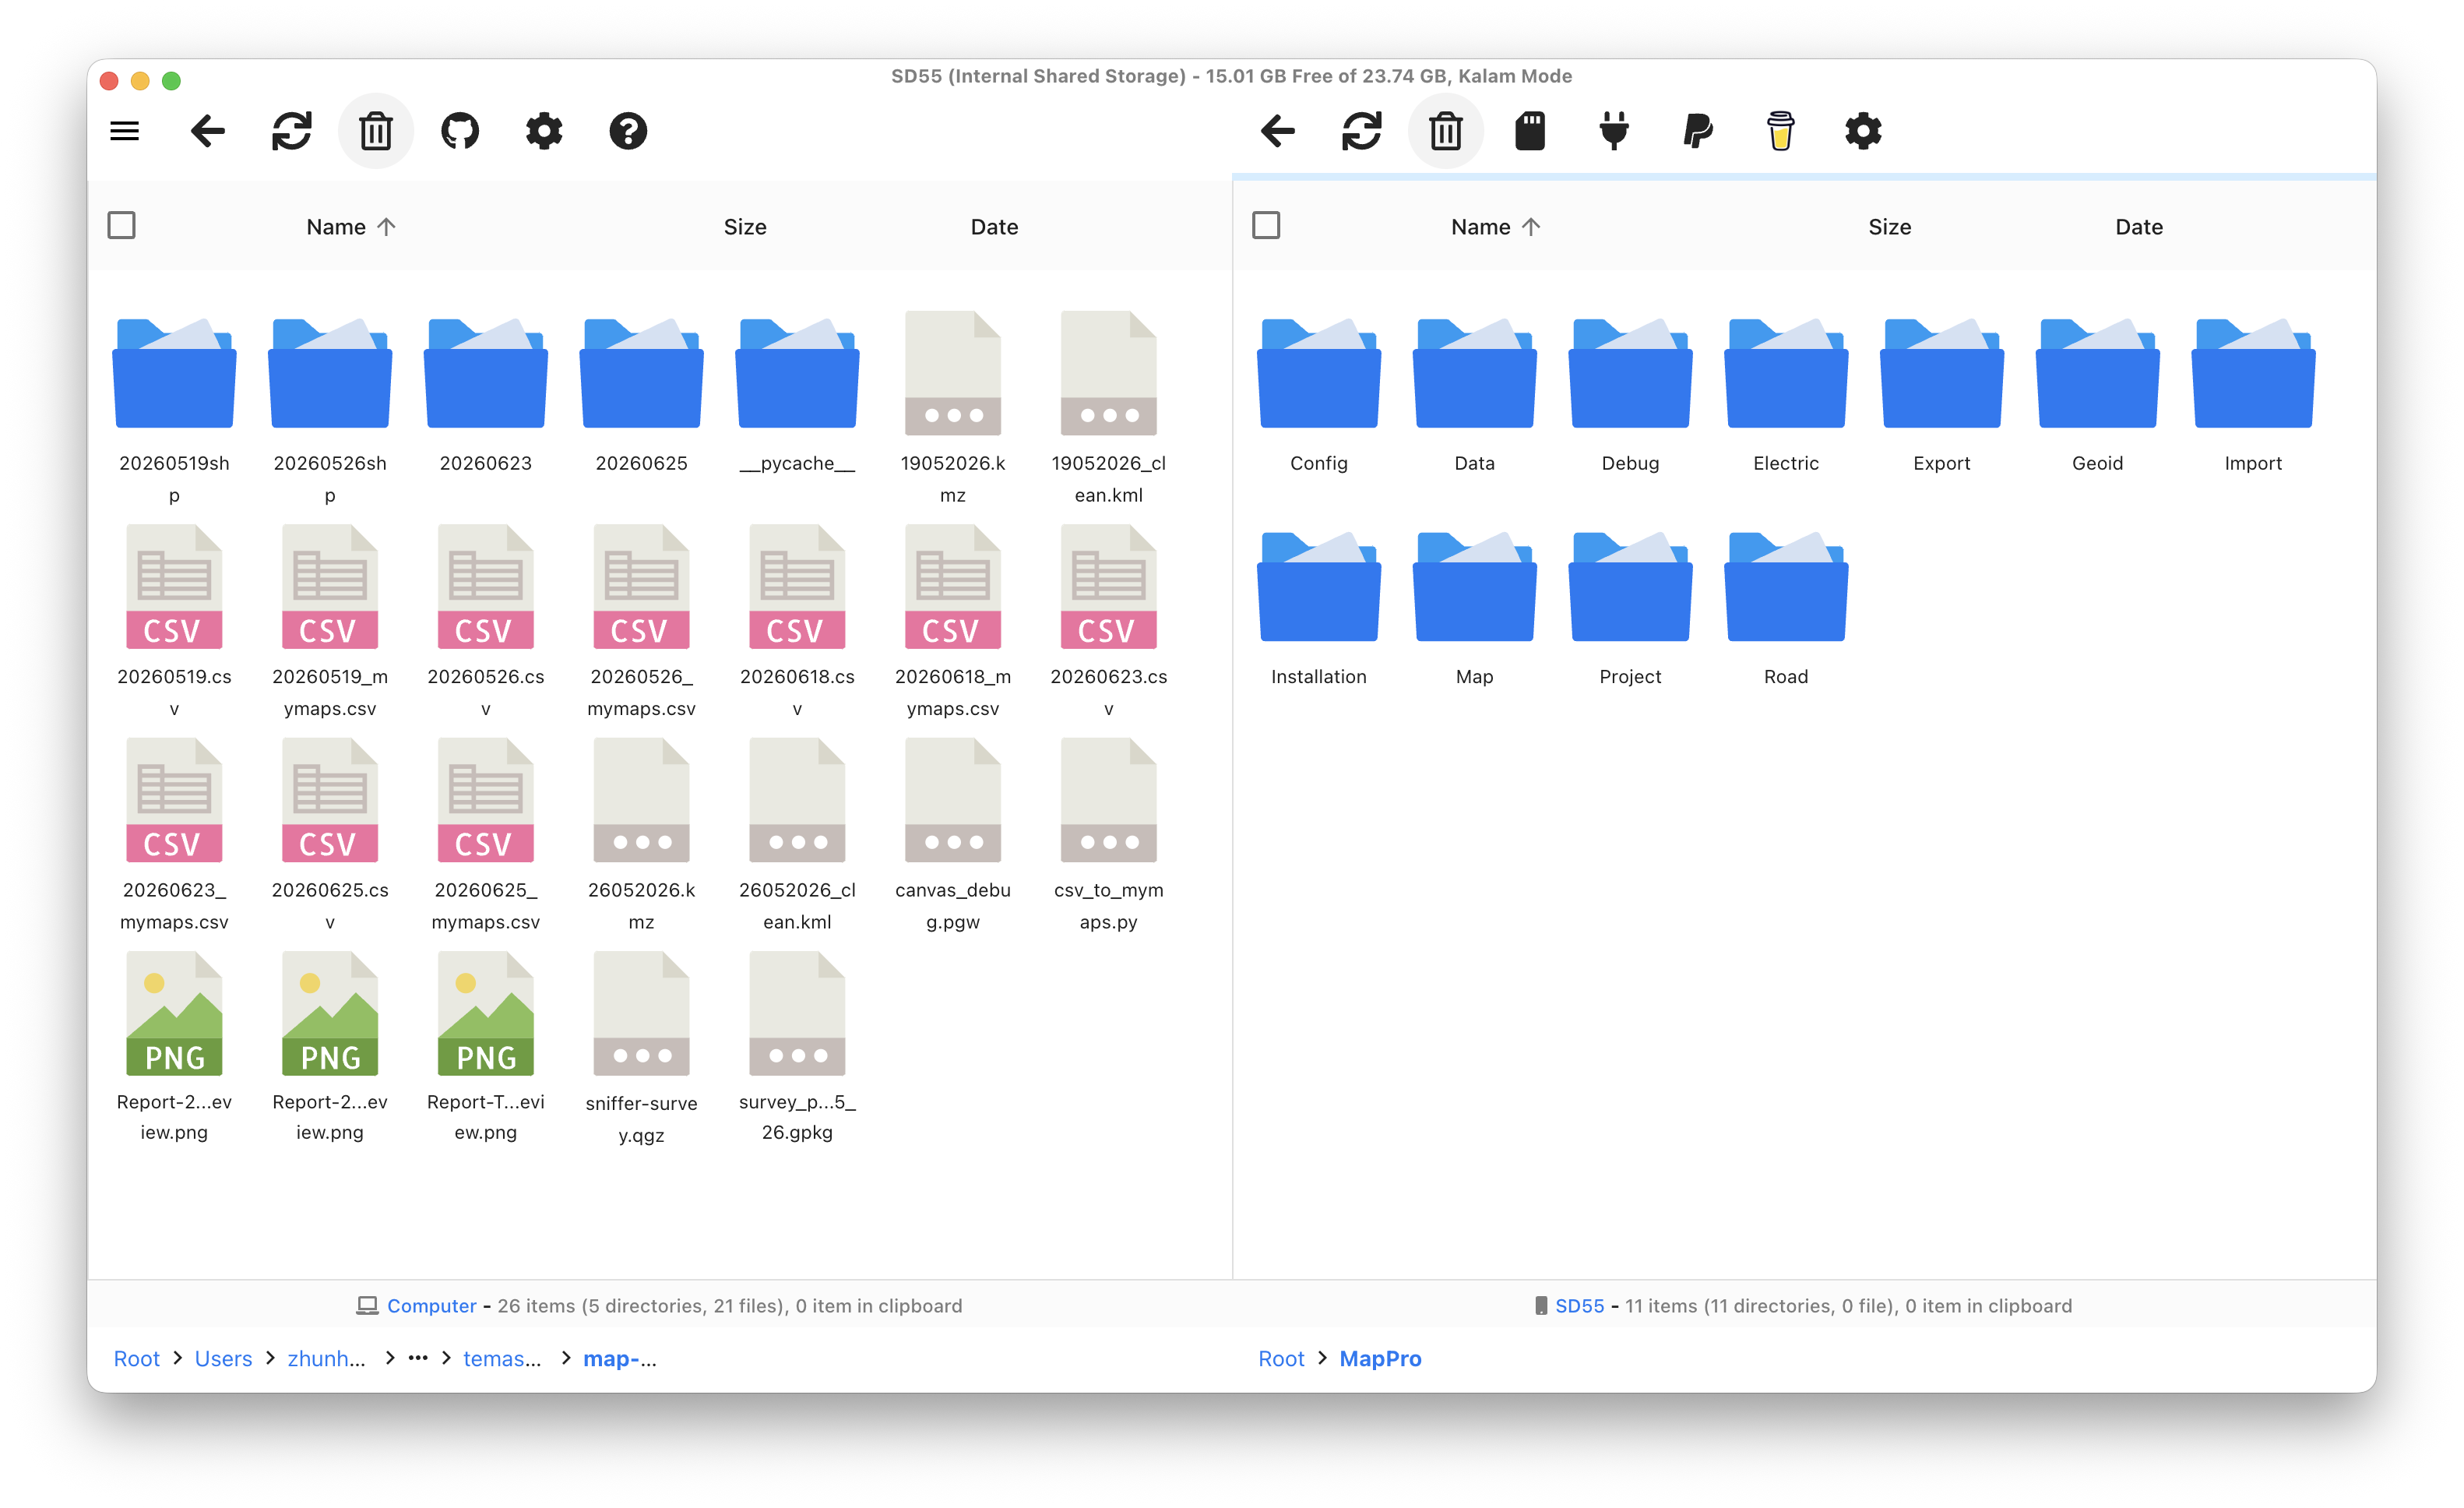
\includegraphics[width=0.85\textwidth]{images/step_2_go_export.png}
    \caption*{Navigating to the Export directory inside OpenMTP.}
\end{figure}

\clearpage

\subsection{Step 18: Transfer the Exported CSV File}
In OpenMTP's device pane (inside the Export folder), locate the survey CSV file you exported (e.g., \texttt{20260626.csv}). Use OpenMTP's local file explorer pane (on the other side) or drag and drop to transfer this file into the local project directory on your laptop (specifically, the \texttt{/Users/zhunhao/Documents/Projects/temasek-lab/map-data-plot/} directory).

\begin{figure}[H]
    \centering
    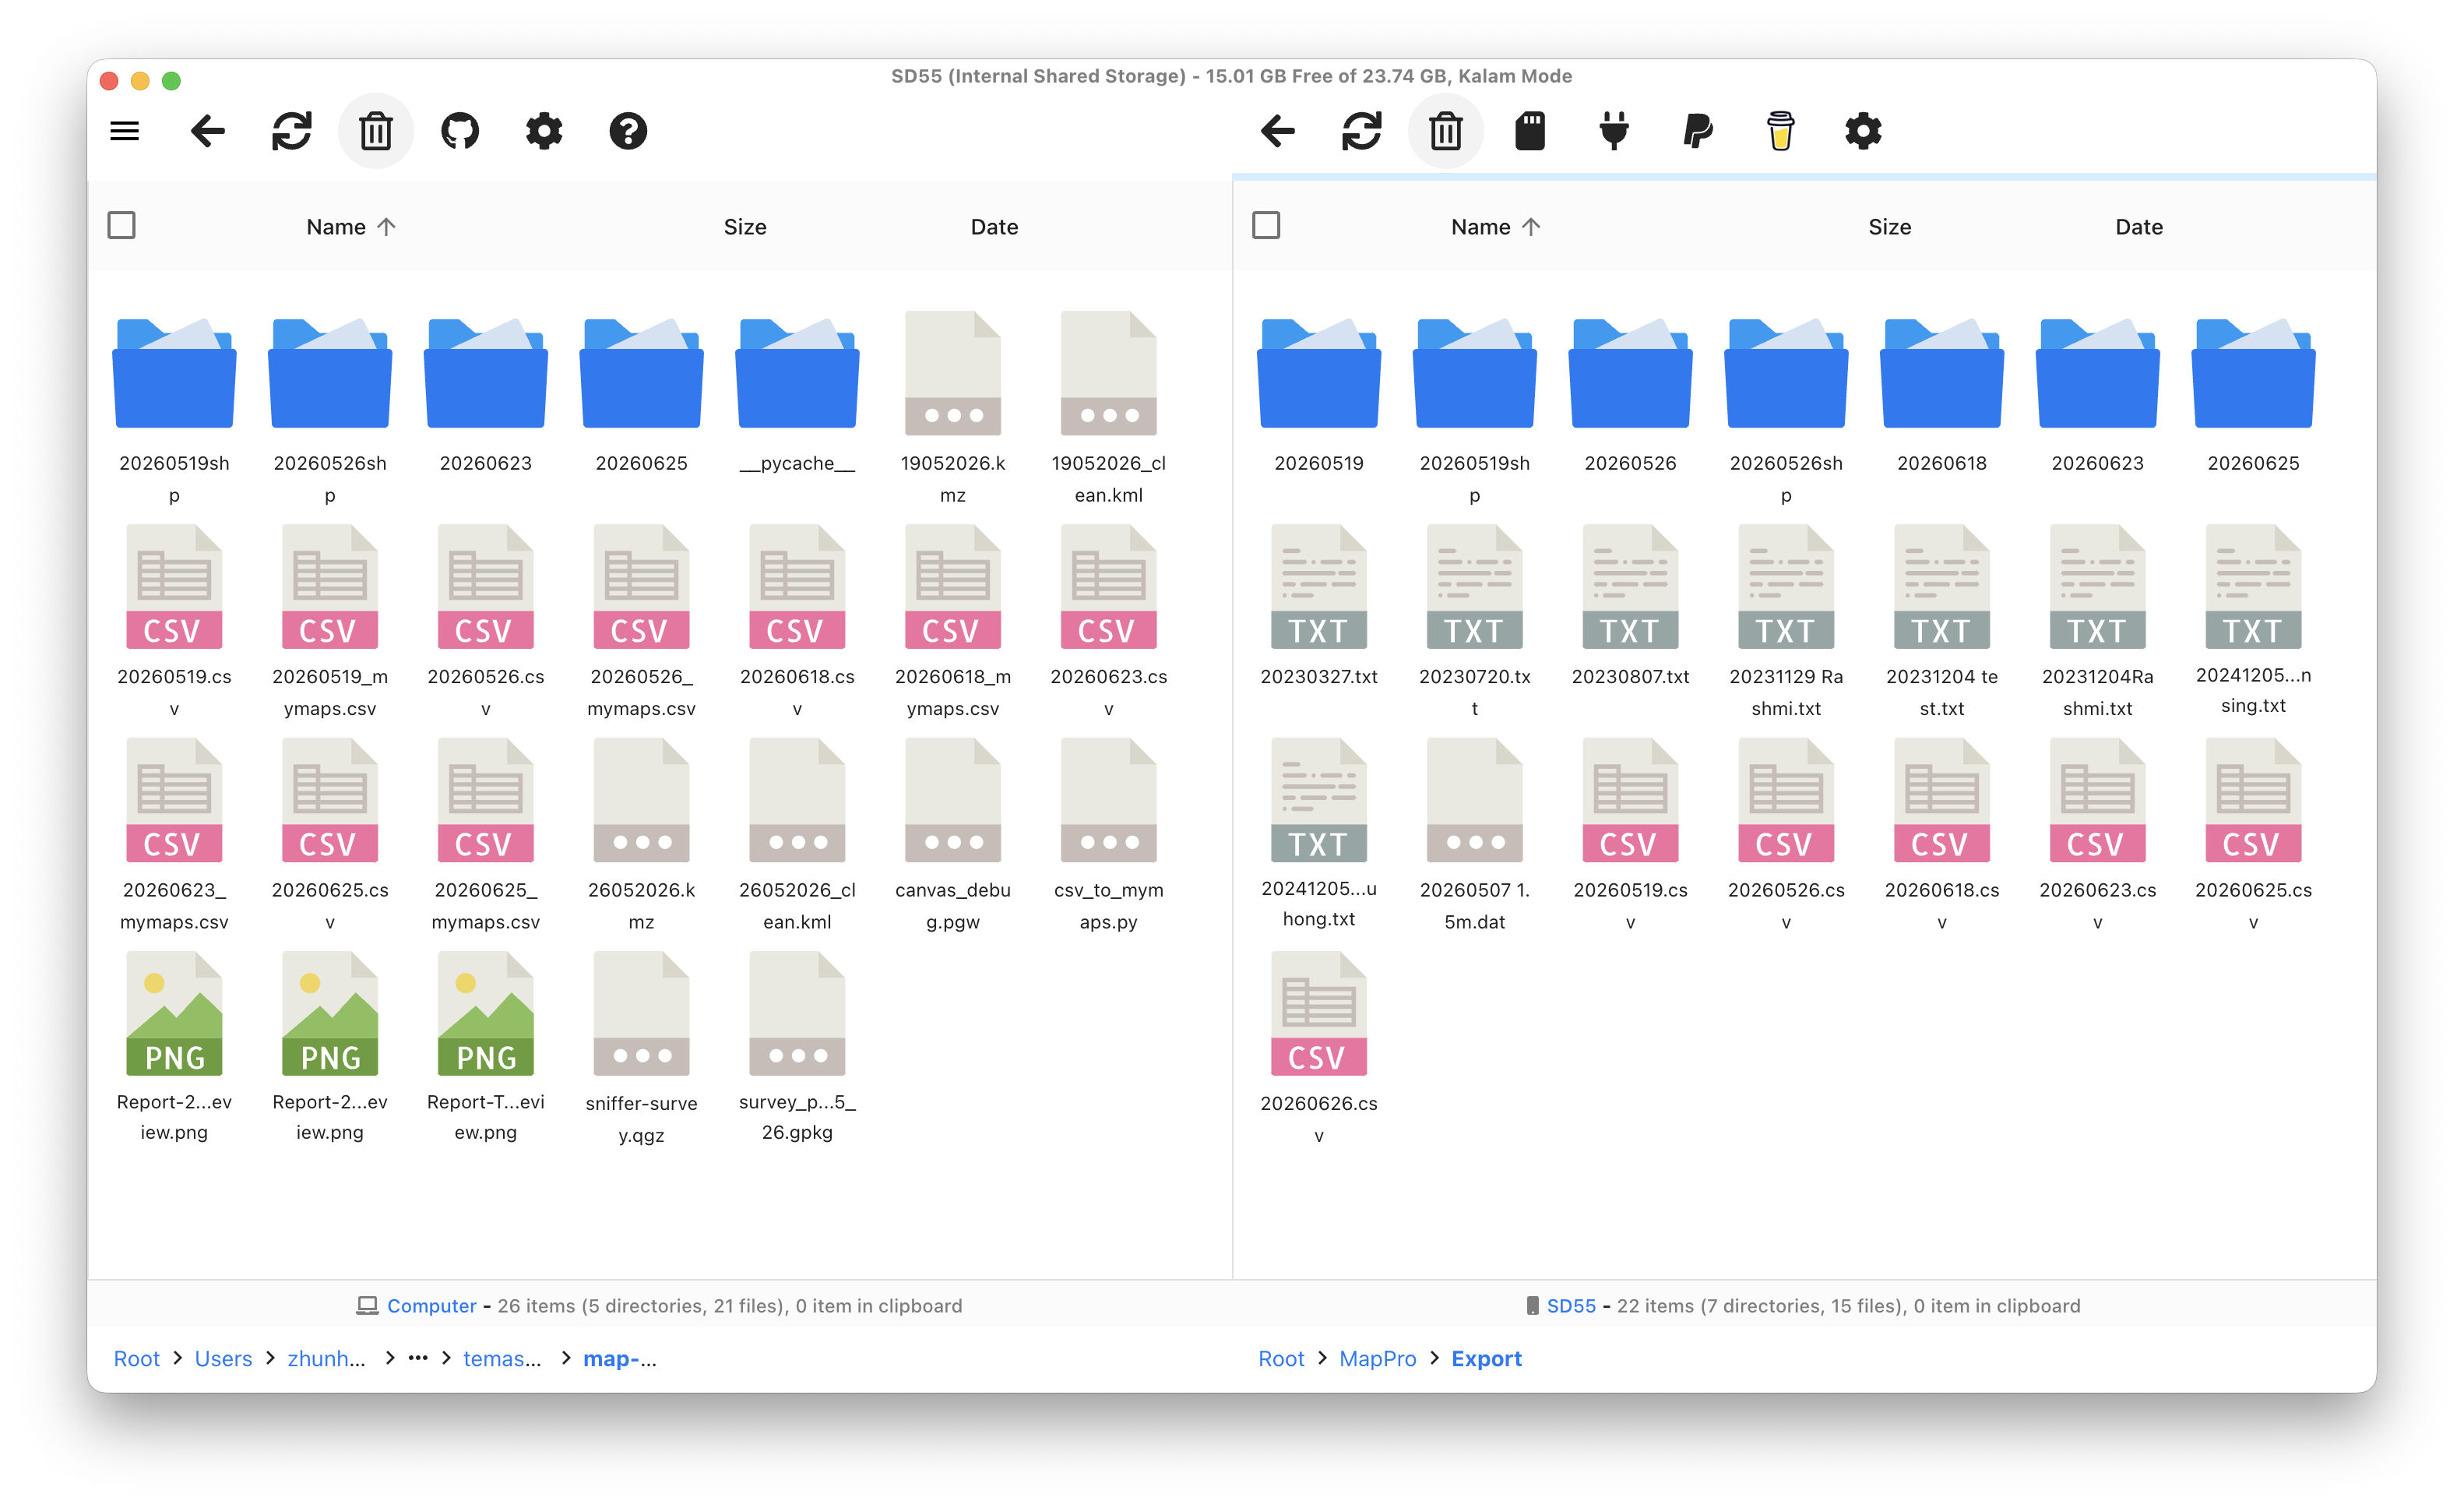
\includegraphics[width=0.85\textwidth]{images/transfer_your_csv_file.png}
    \caption*{Locating the exported survey CSV in OpenMTP and transferring it to the local laptop project folder.}
\end{figure}

\subsection{Step 19: Open Terminal and Navigate to Project Directory}
Open a terminal window on your laptop and navigate to the project directory containing the python script \texttt{csv\_to\_mymaps.py} by executing:

\begin{lstlisting}[language=bash]
cd Documents/Projects/temasek-lab/map-data-plot
\end{lstlisting}

\begin{figure}[H]
    \centering
    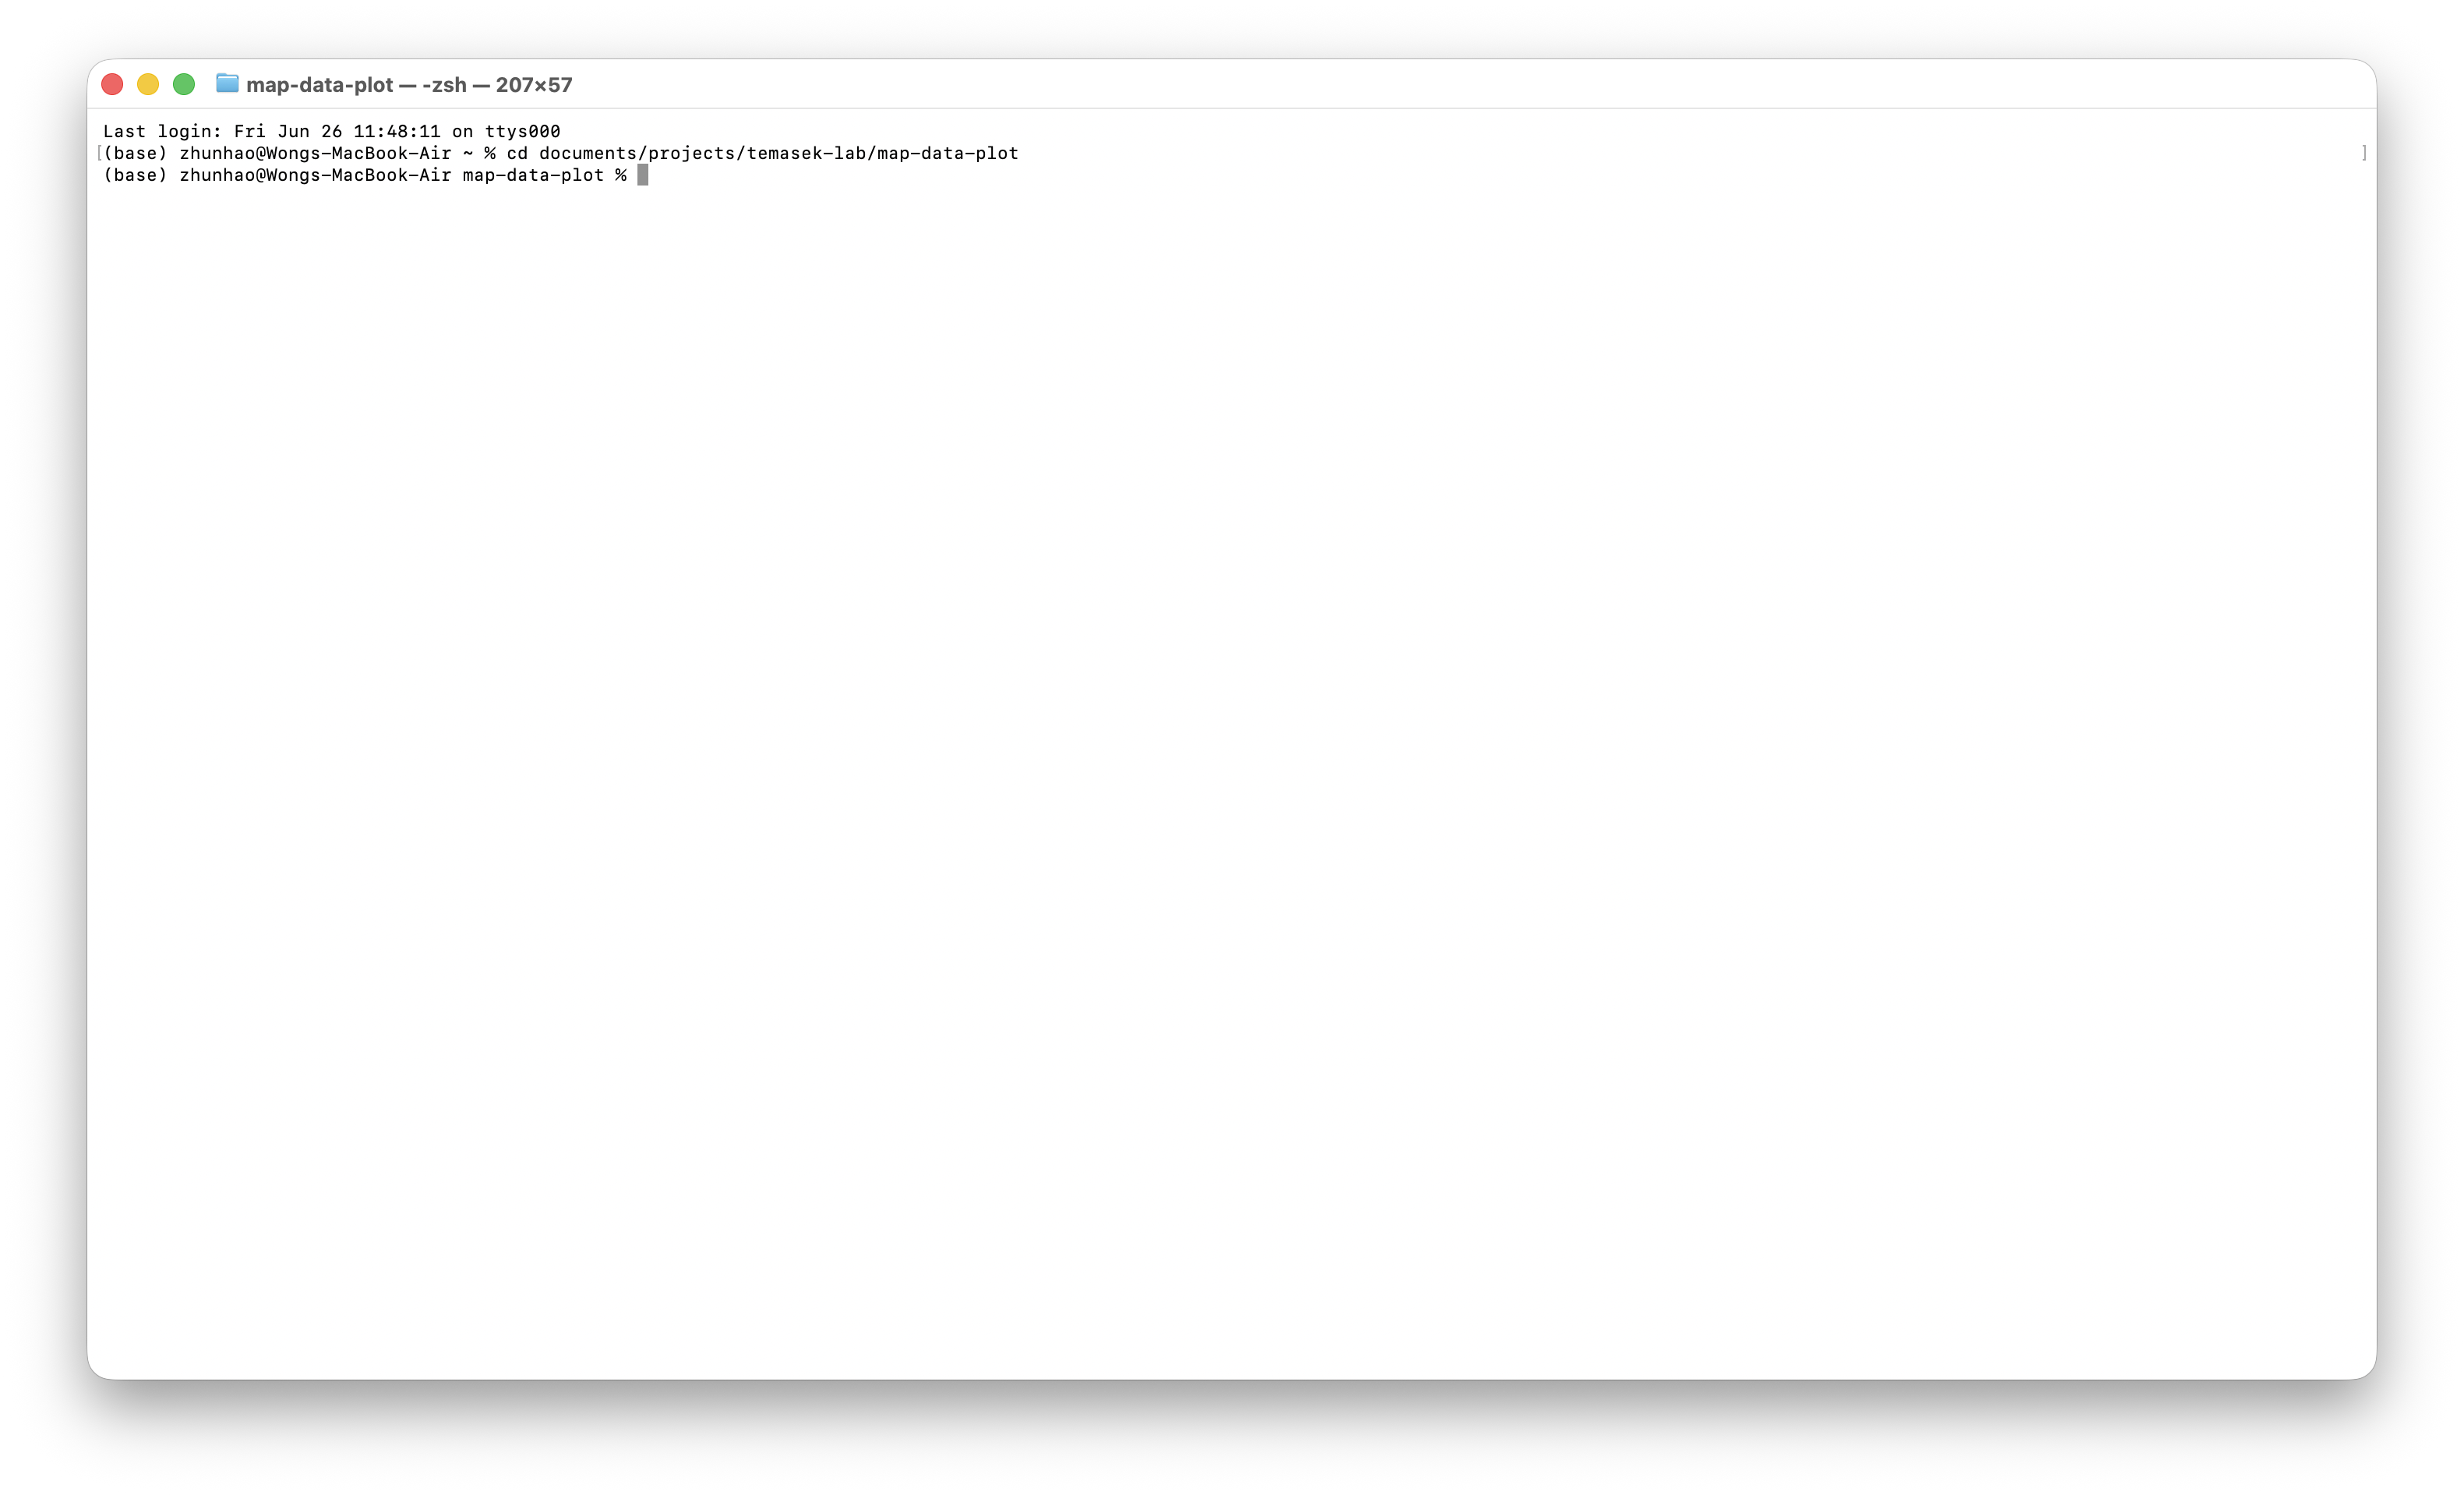
\includegraphics[width=1.0\textwidth]{images/navigate_to_path.png}
    \caption*{Terminal window demonstrating navigation to the project folder.}
\end{figure}

\clearpage

% =========================================================
\section{Coordinate Translation \& Uploading}
% =========================================================

\subsection{Step 20: Translate Packed DMS to Decimal Degrees}
Run the Python script \texttt{csv\_to\_mymaps.py} on the transferred CSV file by typing the following command in your terminal:

\begin{lstlisting}[language=bash]
# Convert a single survey file:
python3 csv_to_mymaps.py 20260626.csv

# Convert multiple survey files simultaneously:
python3 csv_to_mymaps.py file1.csv file2.csv

# View help and usage options:
python3 csv_to_mymaps.py --help
\end{lstlisting}

The script utilizes the \texttt{argparse} library to parse and process your files, replacing the packed Degrees-Minutes-Seconds coordinate values in the columns \textit{Latitude}, \textit{Longitude}, \textit{Original Latitude}, \textit{Original Longitude}, \textit{Base Latitude}, and \textit{Base Longitude} in-place with signed decimal degrees. It writes the sanitized data to a new file named \texttt{20260626\_mymaps.csv} (or \texttt{<filename>\_mymaps.csv}).

\begin{figure}[H]
    \centering
    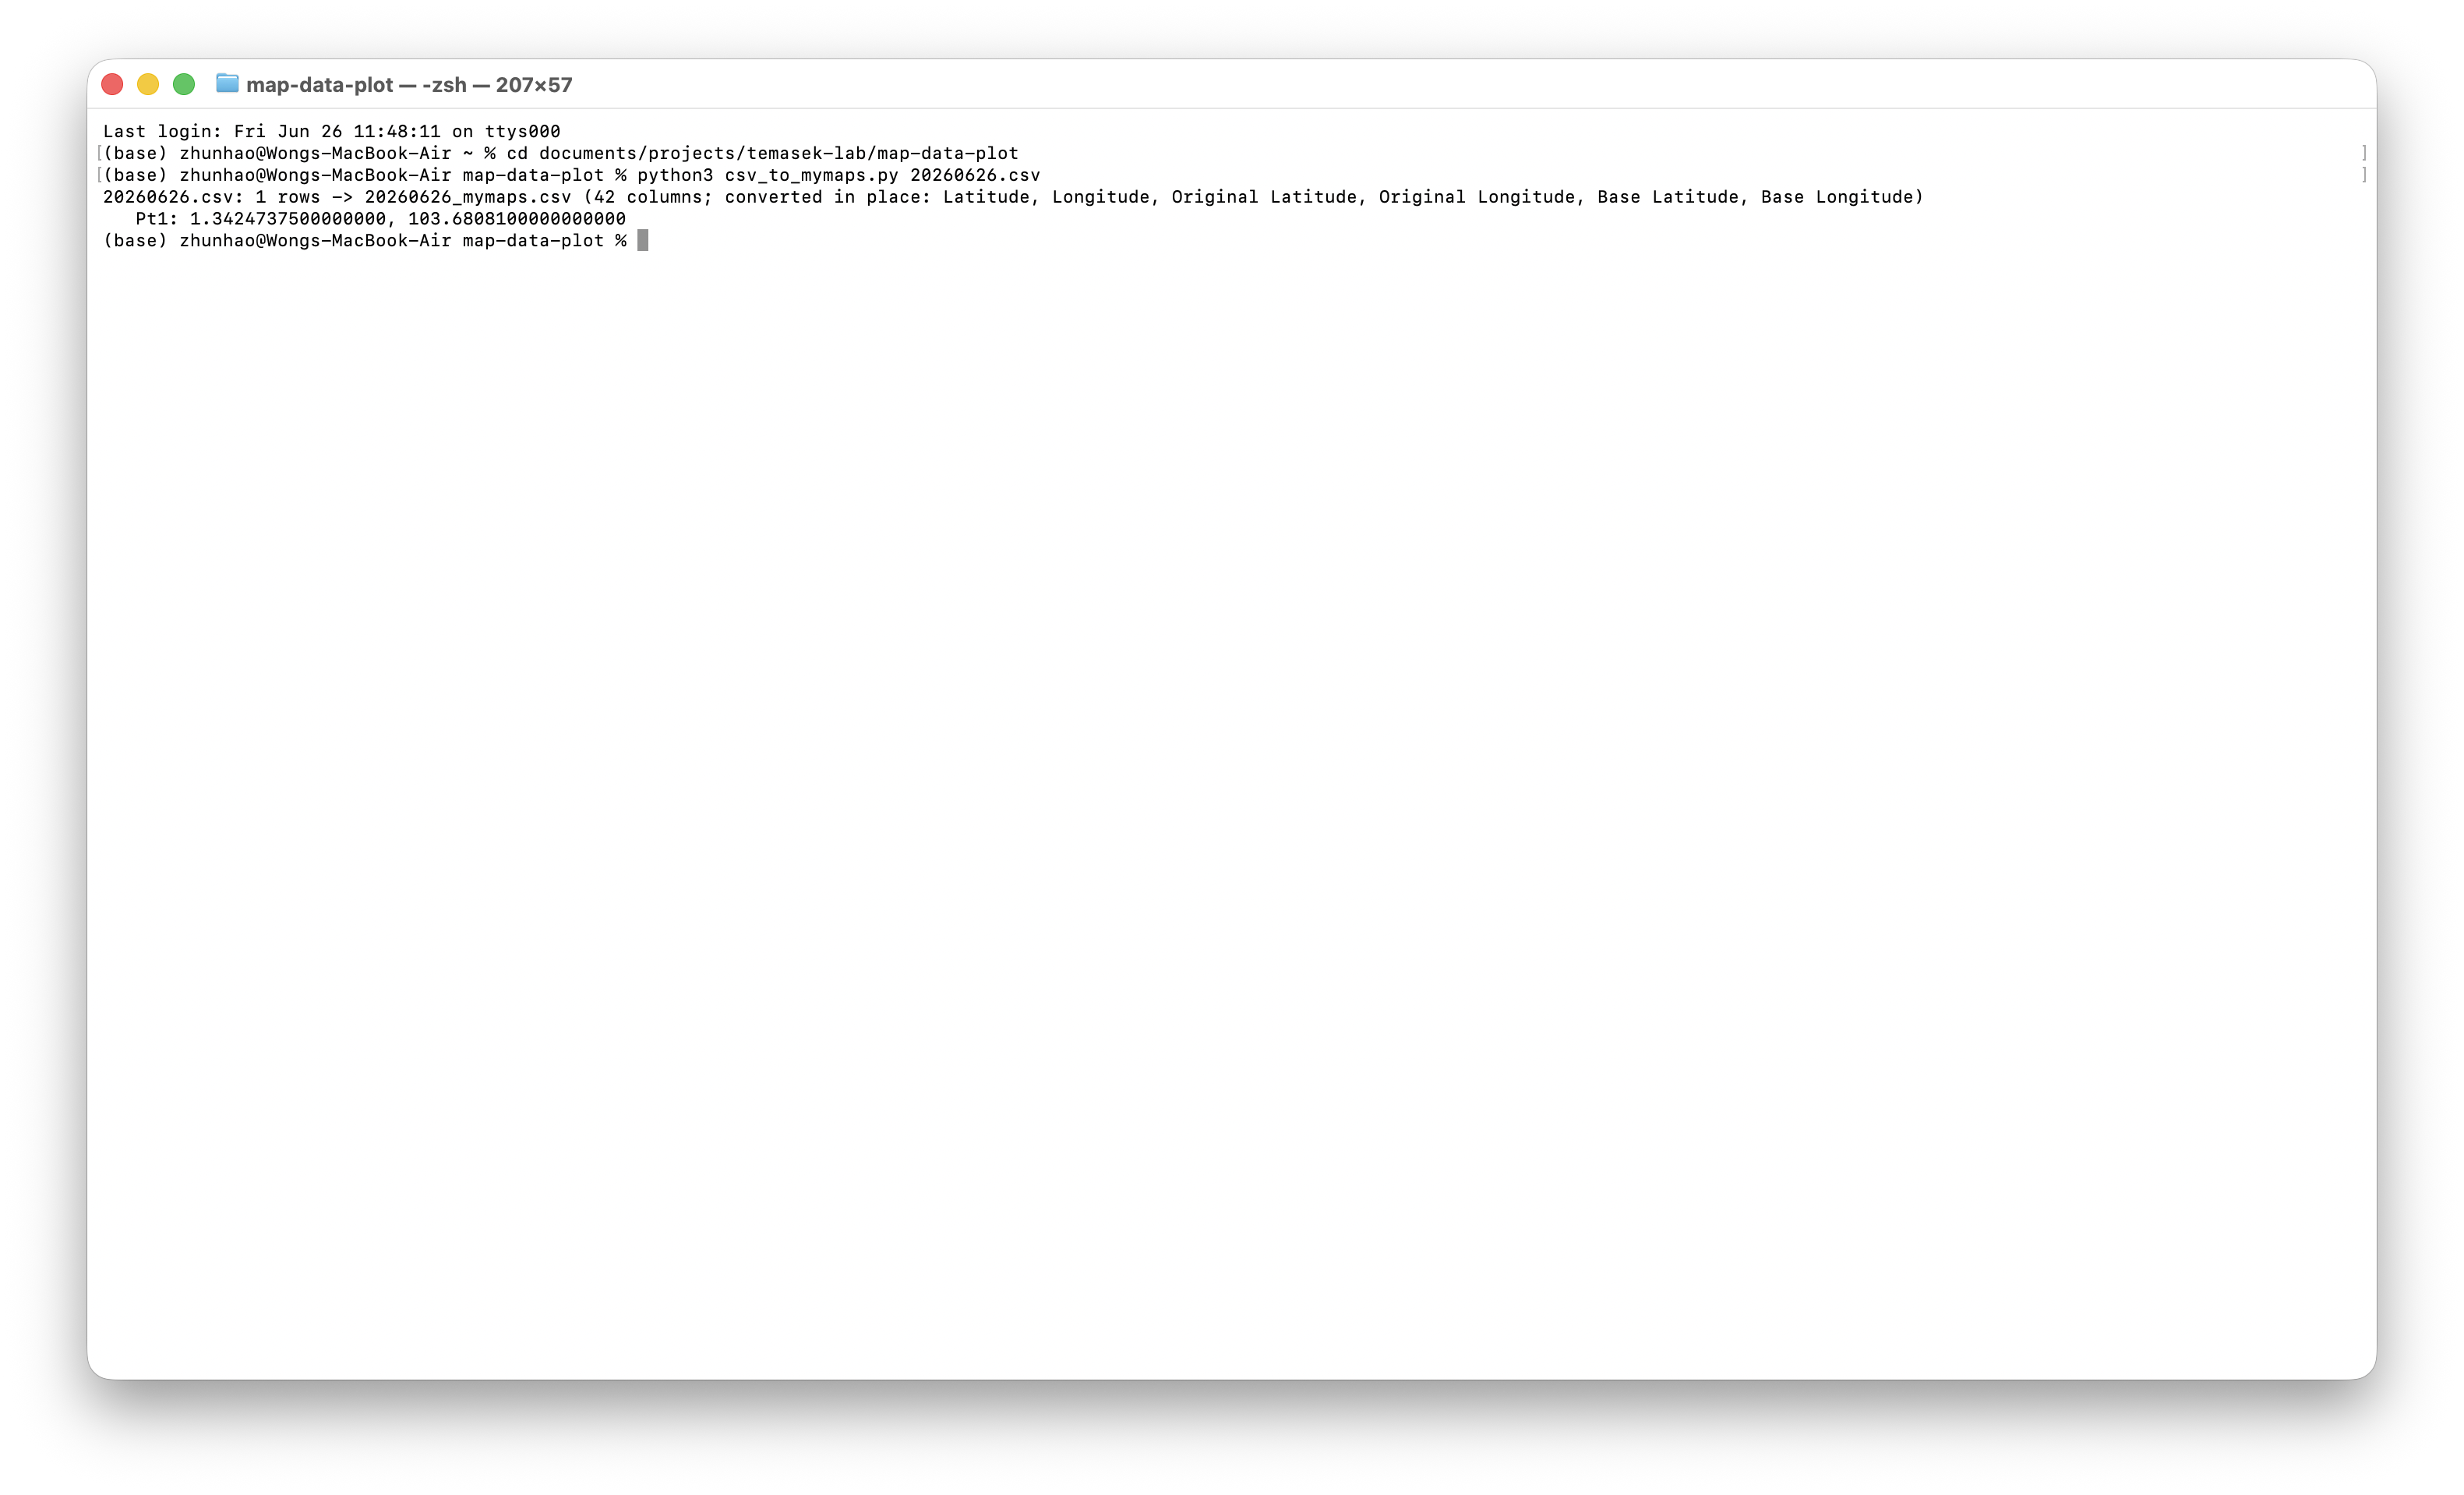
\includegraphics[width=1.0\textwidth]{images/python_script_run.png}
    \caption*{Running the coordinate translation script and outputting decimal degree coordinates.}
\end{figure}

\clearpage

\subsection{Step 21: Navigate to Google My Maps}
Open a web browser on your computer and navigate to \href{https://mymaps.google.com}{mymaps.google.com}. Ensure you are logged into your Google account. You will see your Google My Maps dashboard.

\begin{figure}[H]
    \centering
    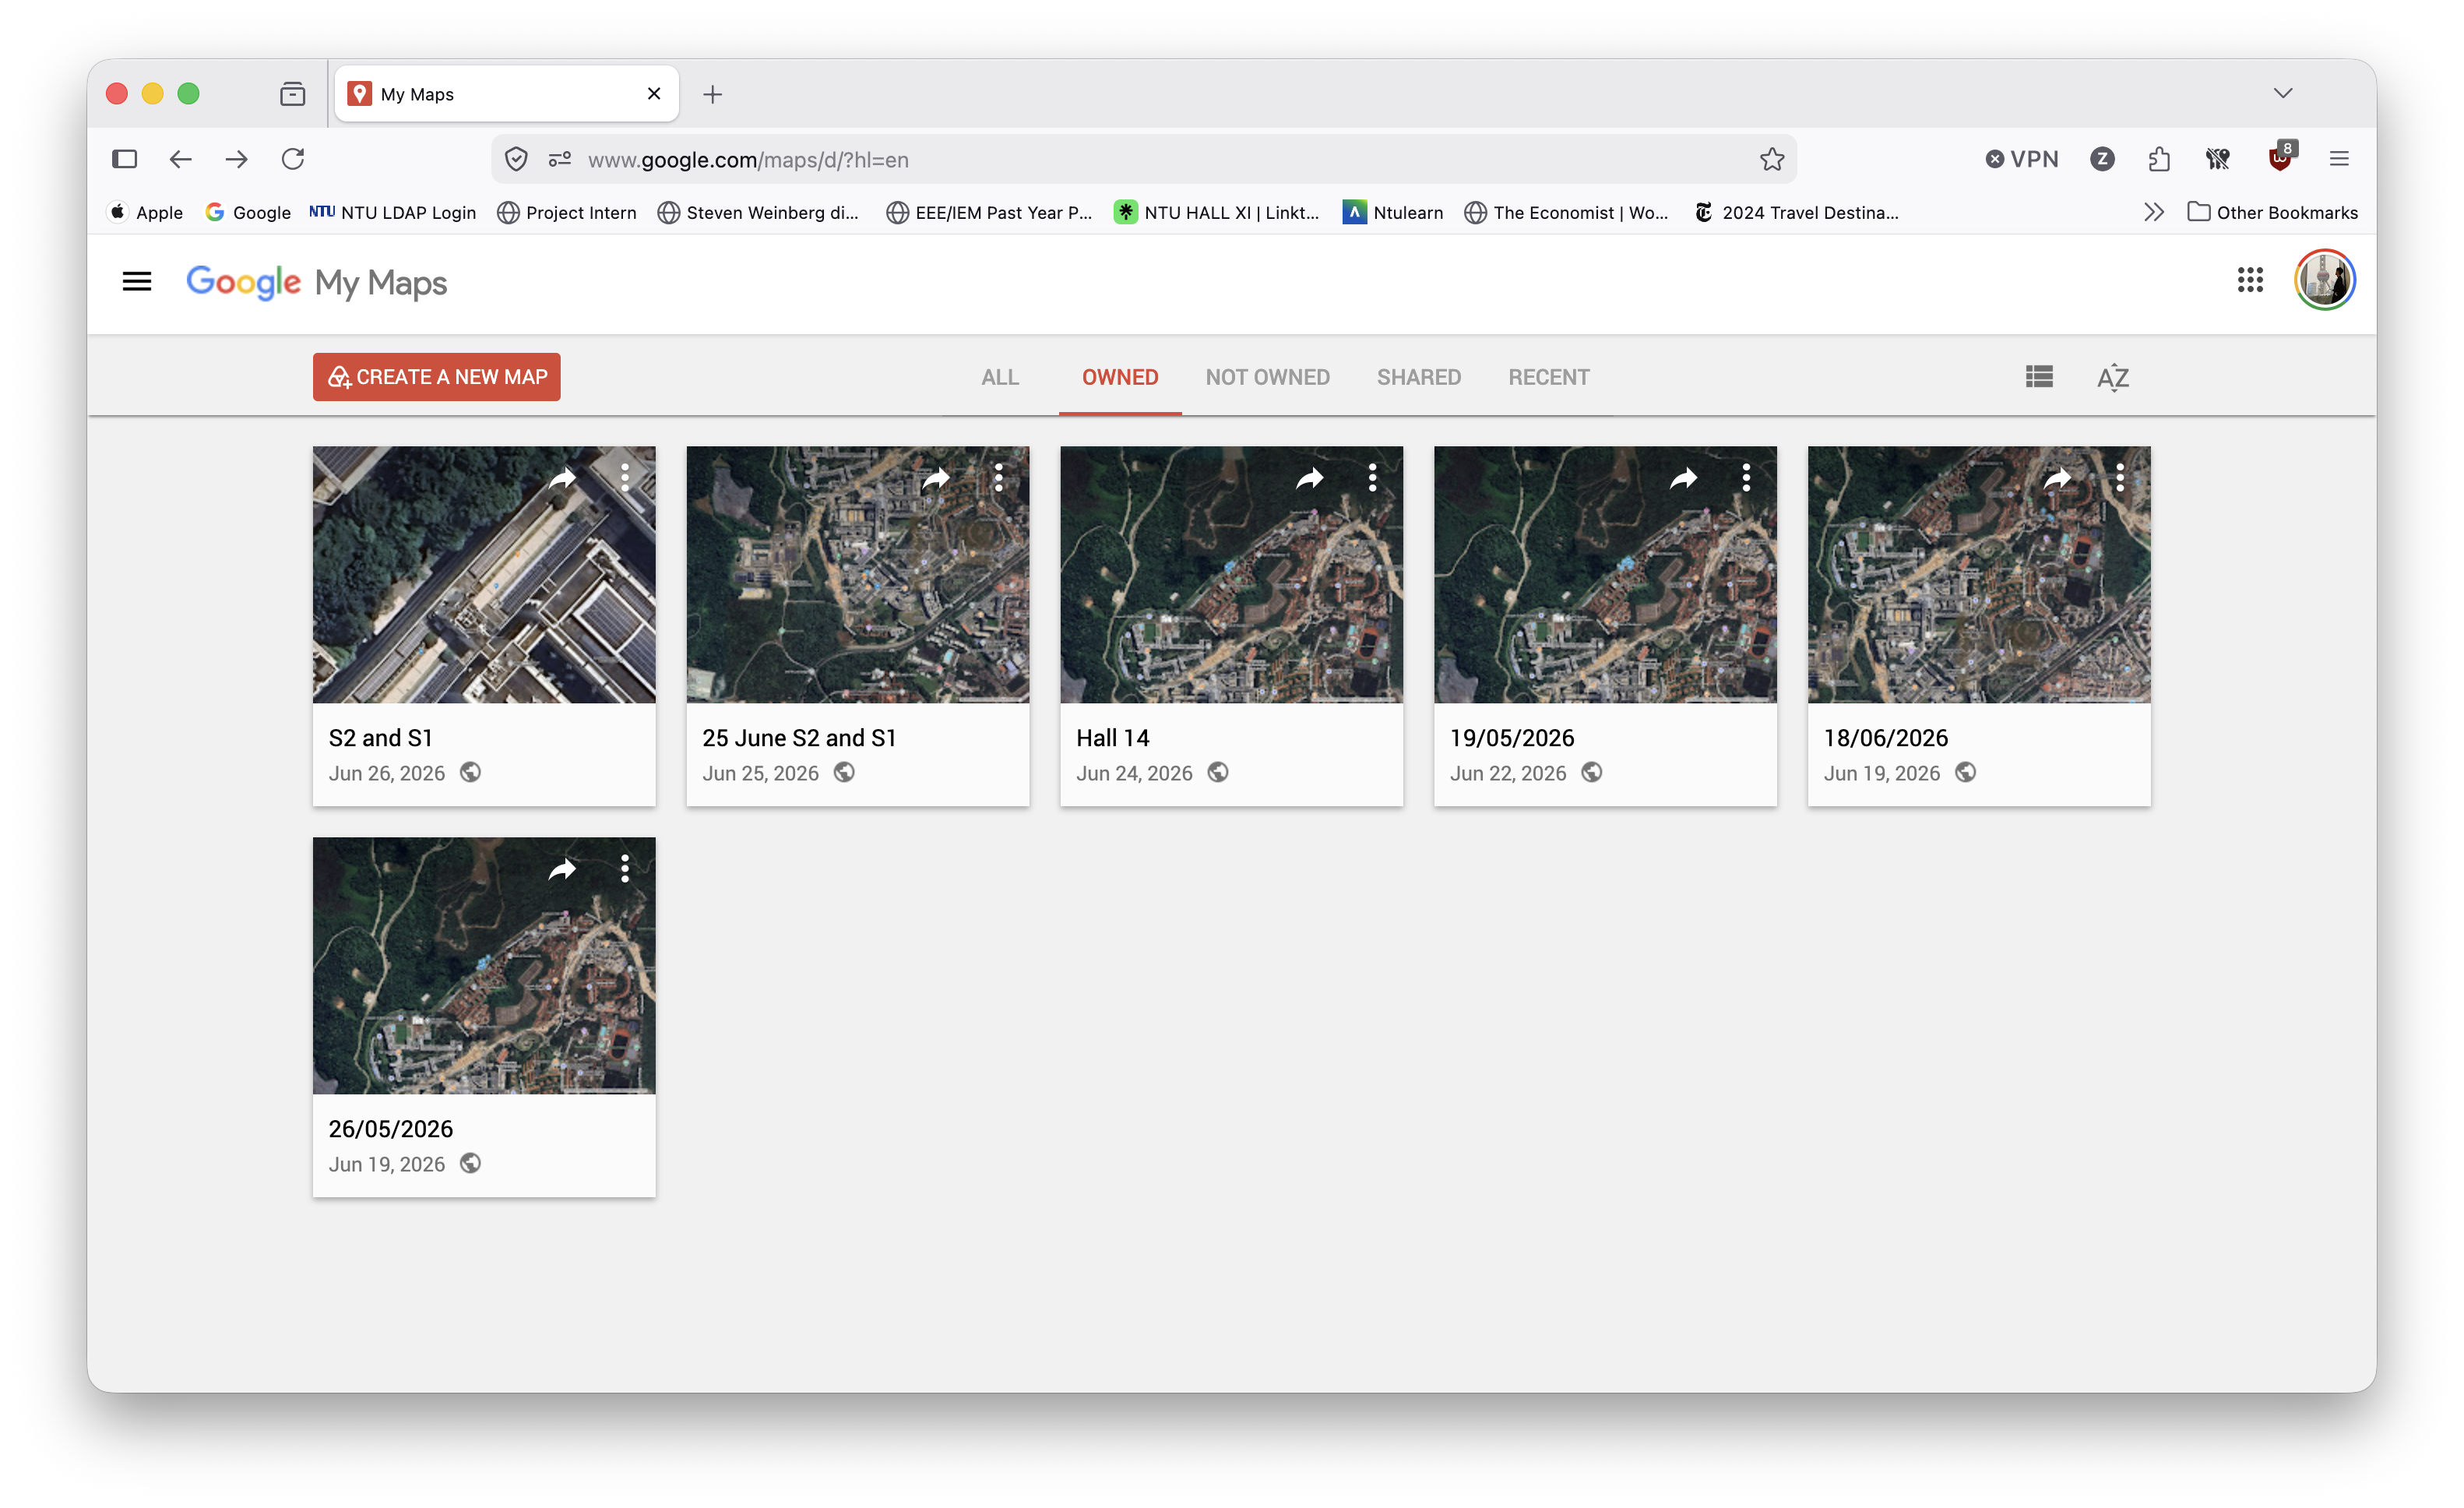
\includegraphics[width=1.0\textwidth]{images/go_google_mymaps.png}
    \caption*{Google My Maps home dashboard containing existing maps and creation options.}
\end{figure}

\subsection{Step 22: Create a New Map}
Click the red \textbf{Create a new map} button in the top left corner of the dashboard to open a blank map project.

\begin{figure}[H]
    \centering
    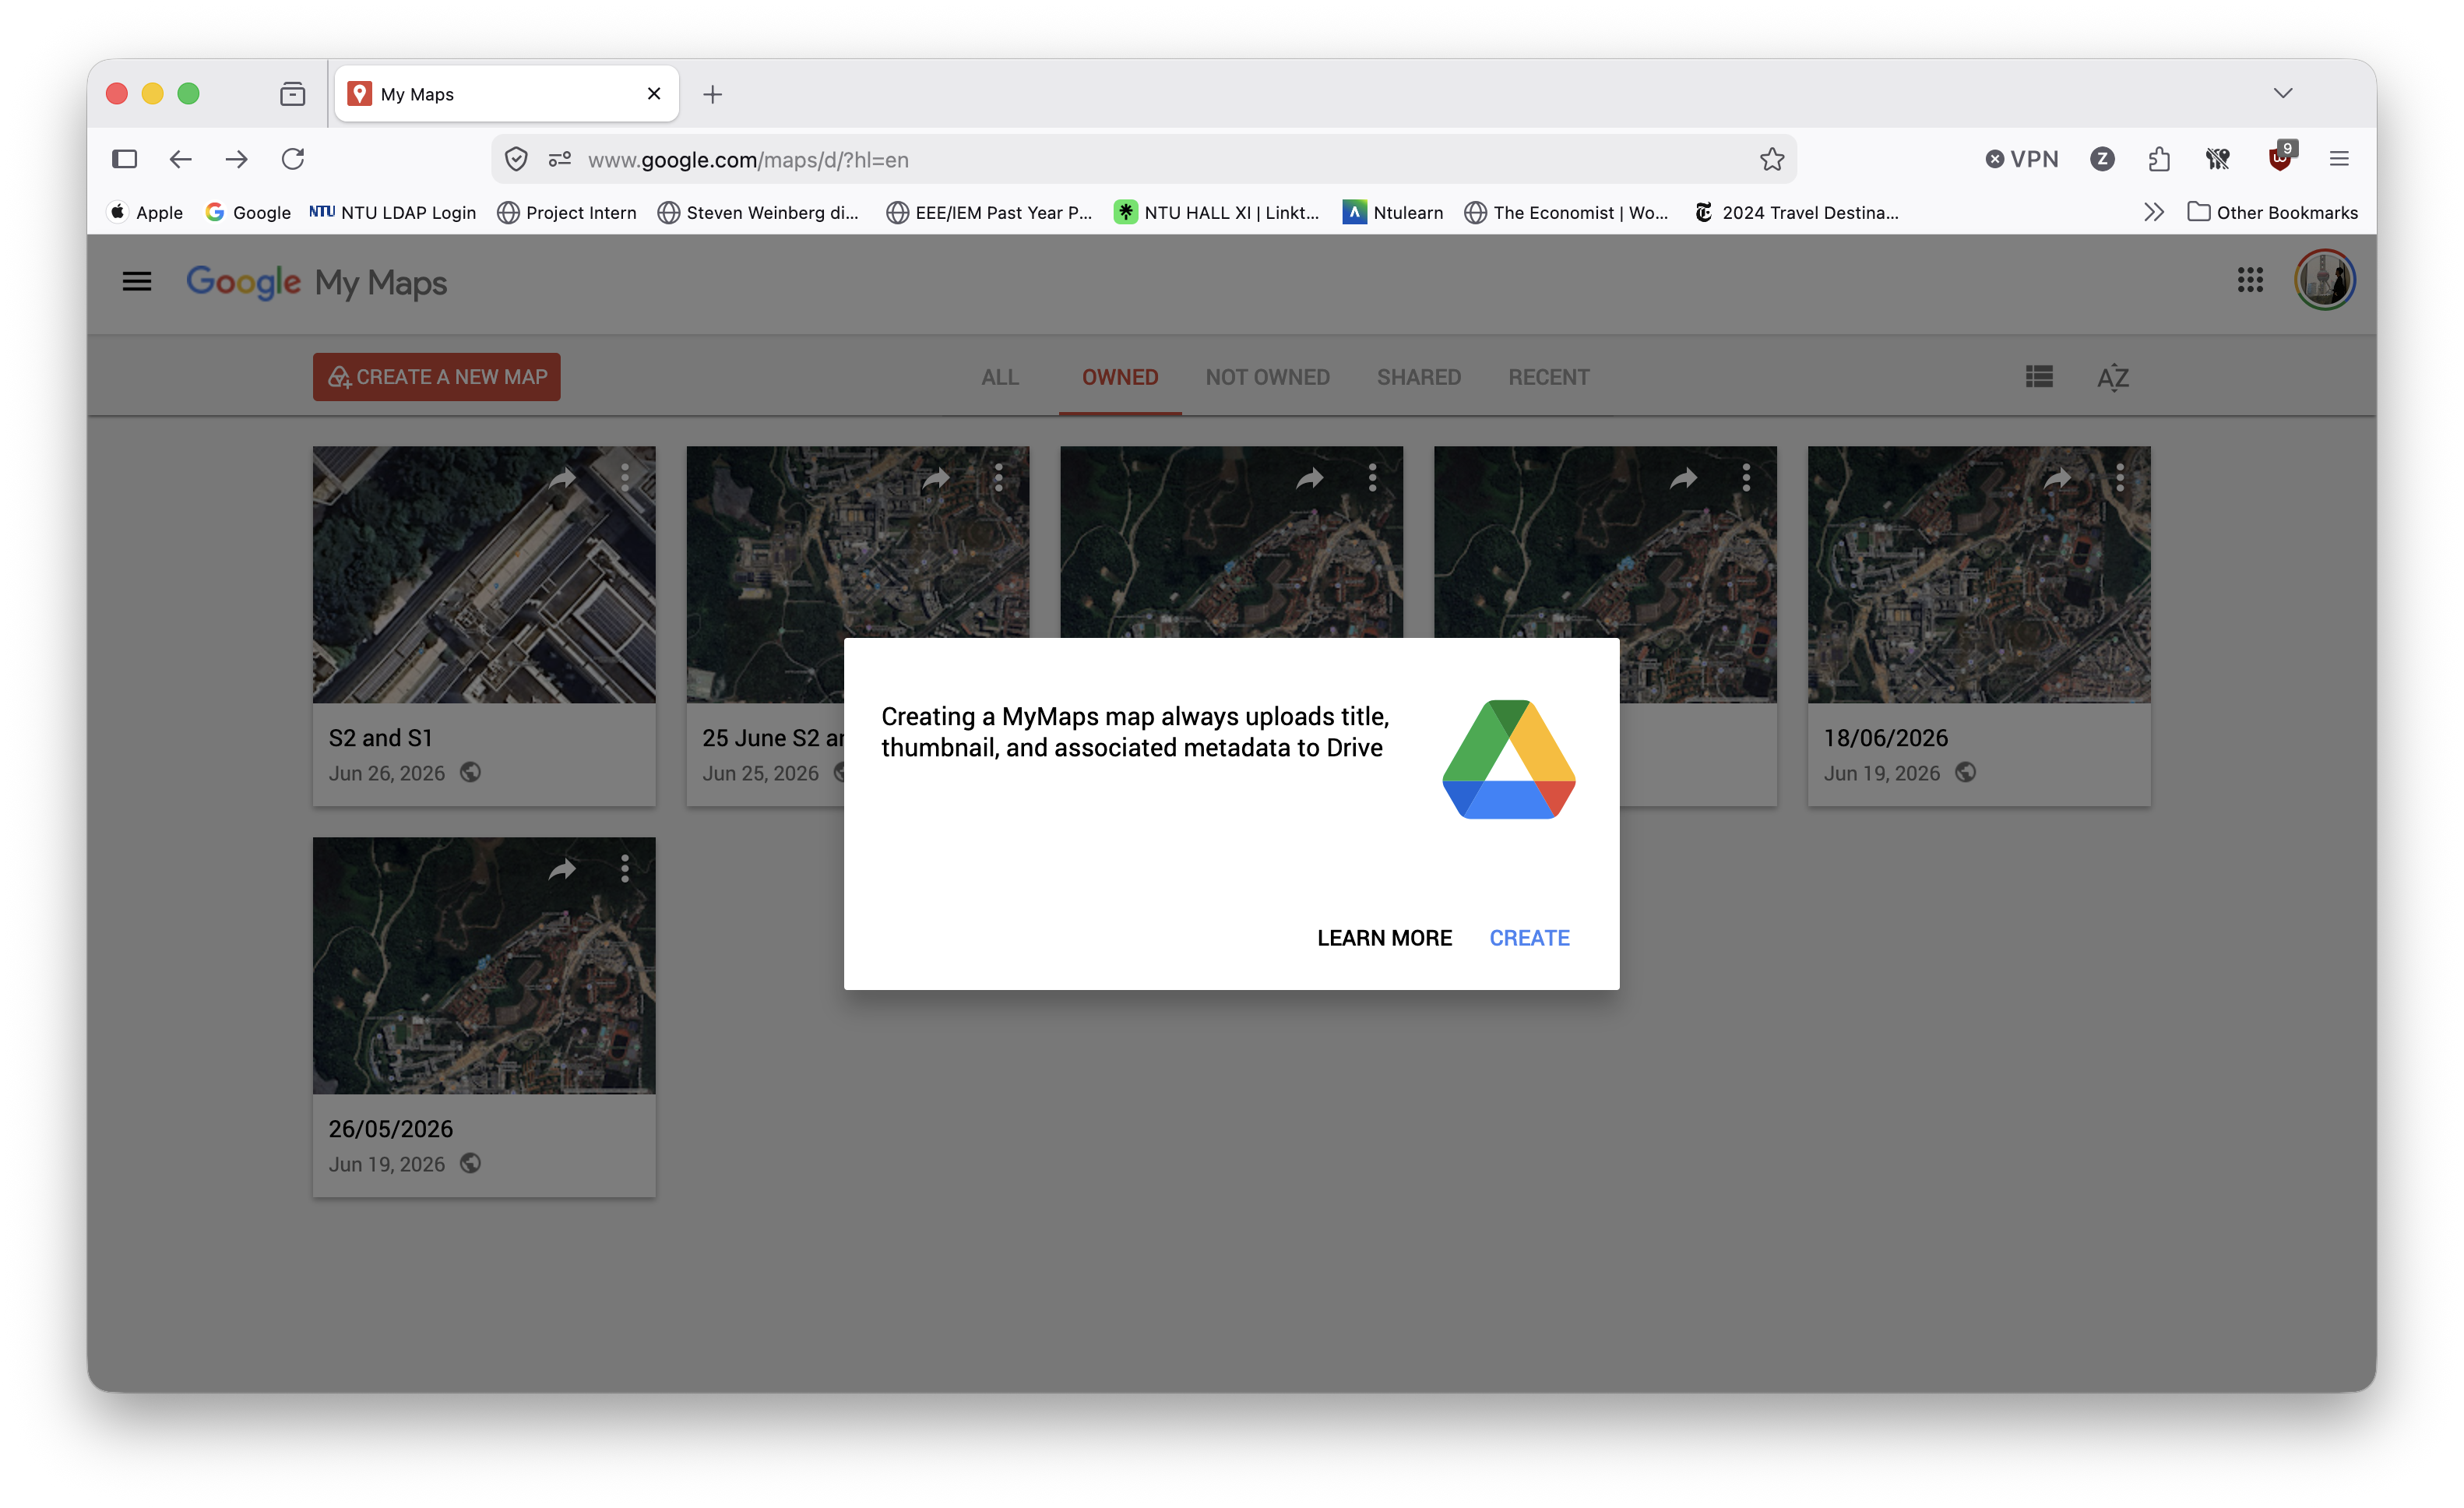
\includegraphics[width=1.0\textwidth]{images/create_a_new_maps.png}
    \caption*{Initializing a new, untitled project in Google My Maps.}
\end{figure}

\clearpage

\subsection{Step 23: Toggle Satellite Base Map}
To view the points over aerial imagery rather than standard map vectors, click the \textbf{Base map} dropdown arrow at the bottom of the layer panel and select the \textbf{Satellite} style.

\begin{figure}[H]
    \centering
    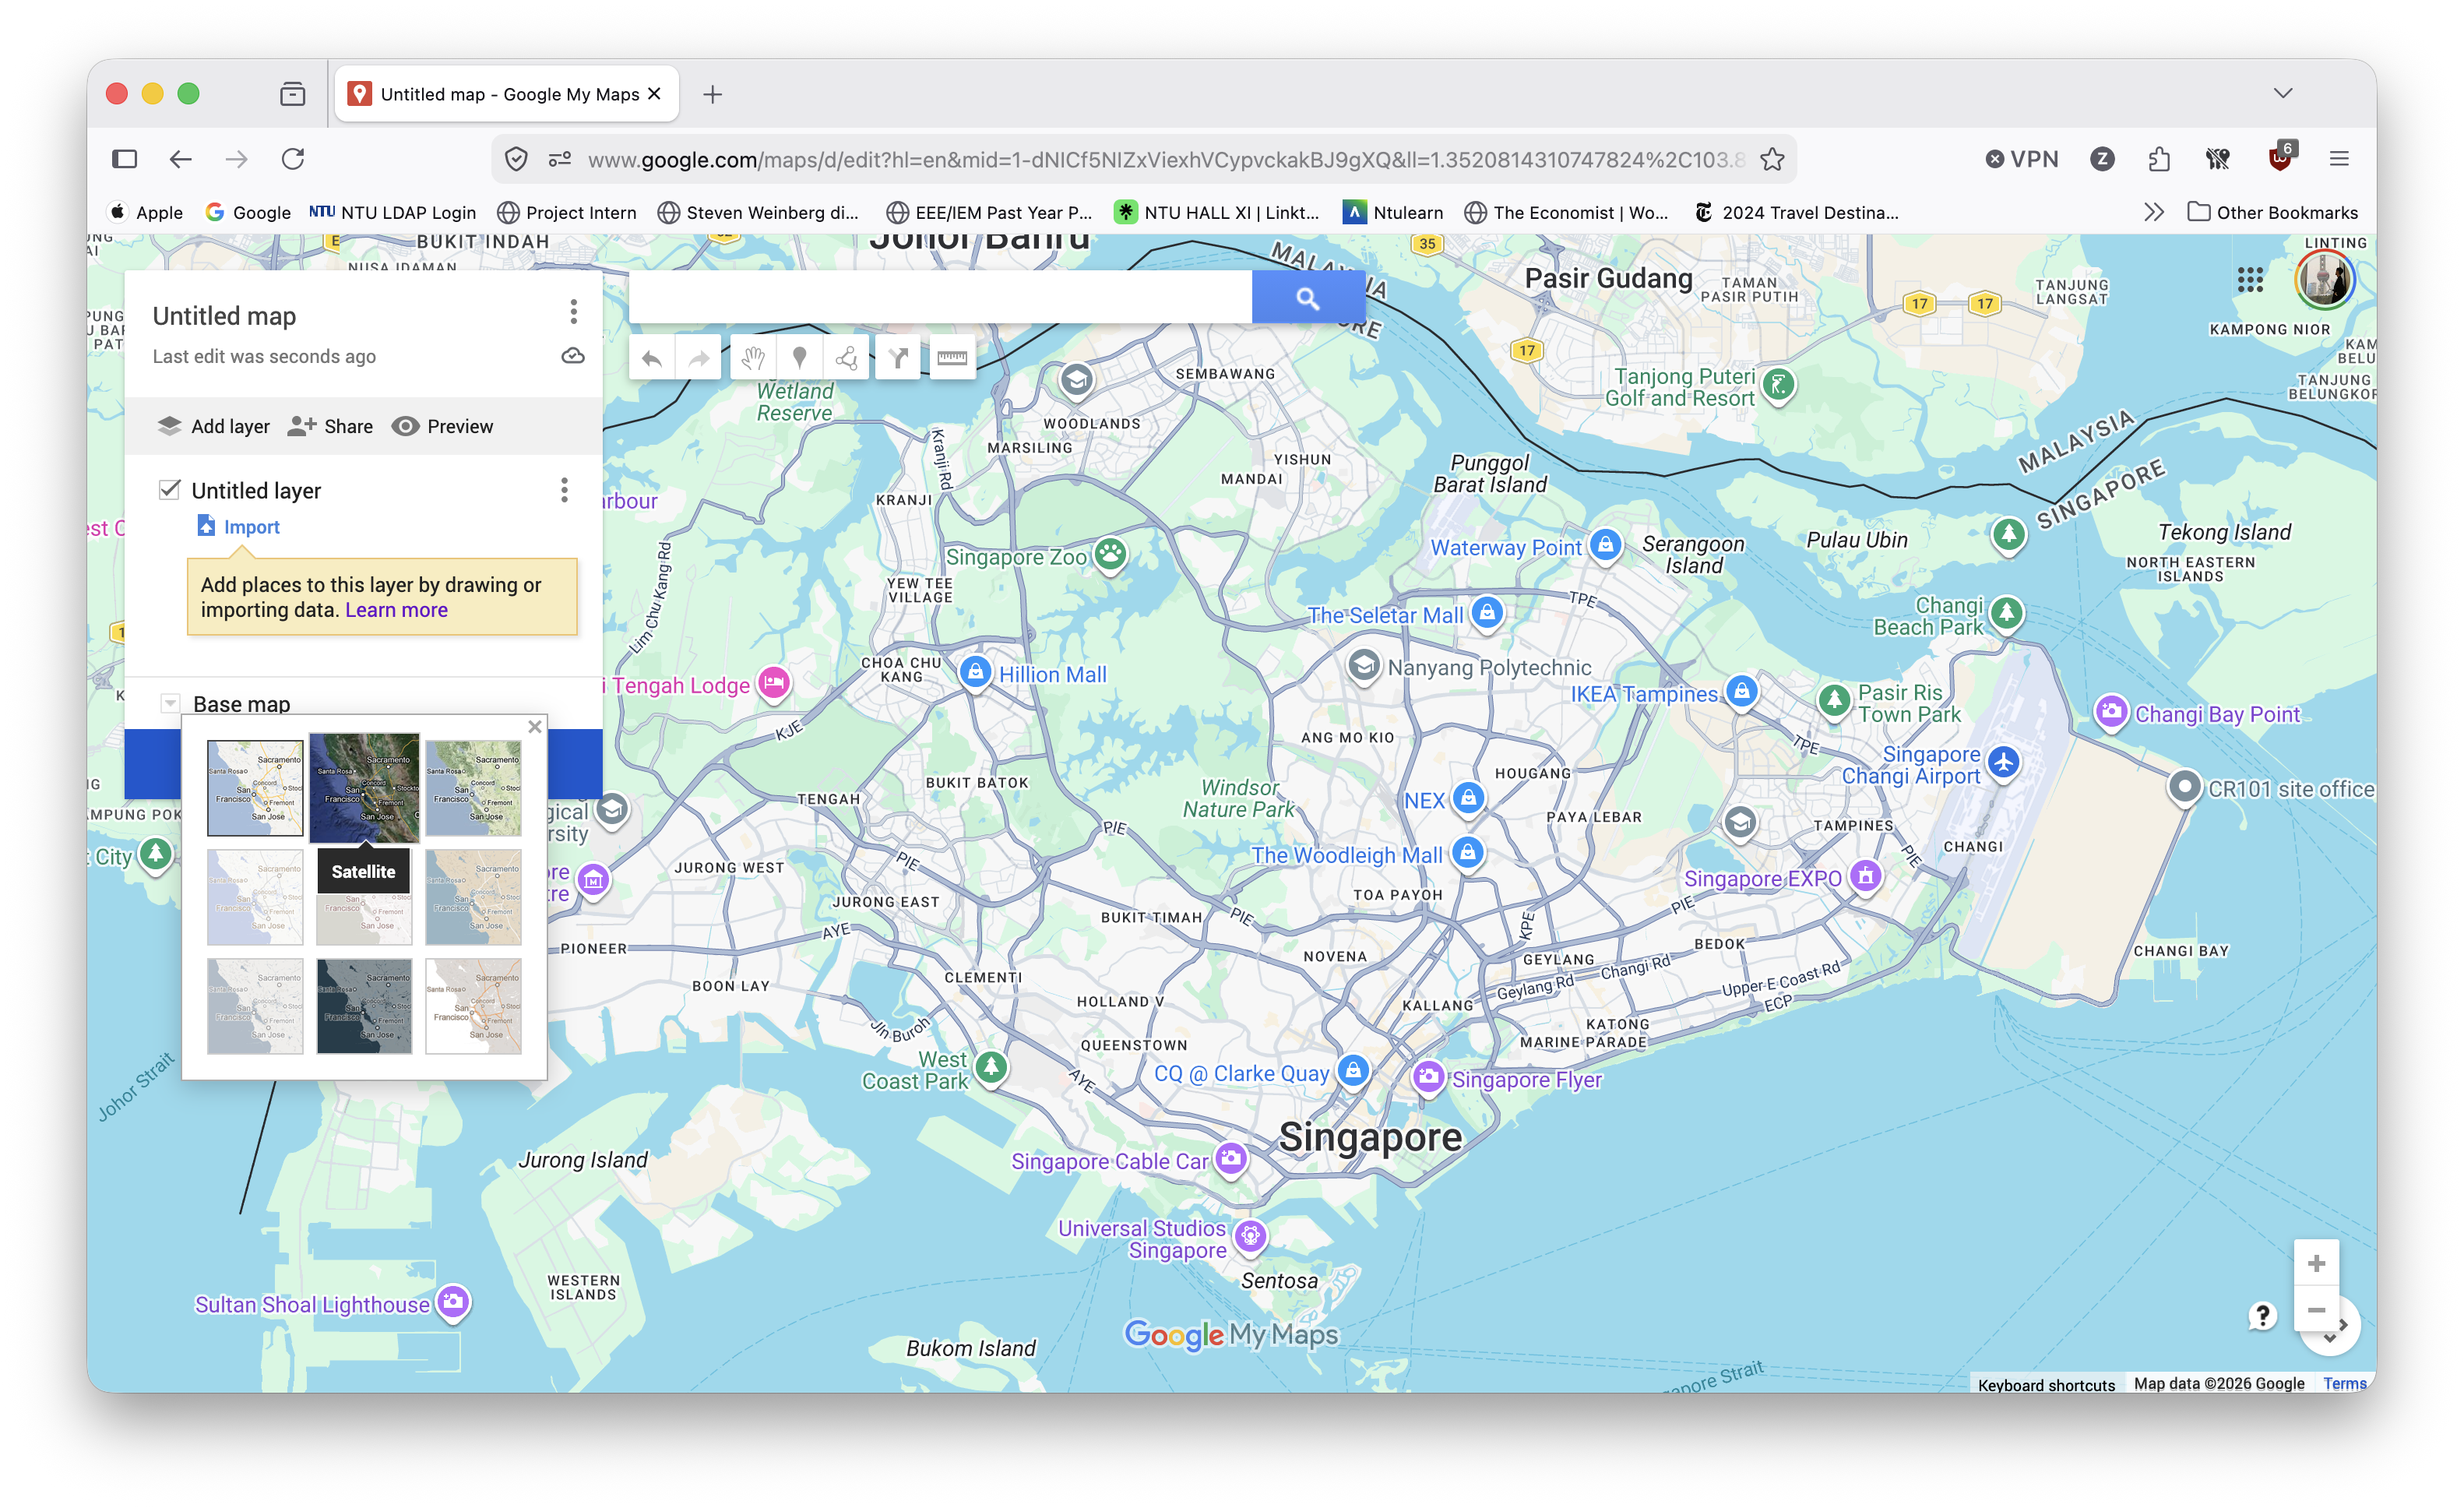
\includegraphics[width=1.0\textwidth]{images/cahnge_base_map_to_satellite.png}
    \caption*{Toggling the Google My Maps base layer to high-resolution satellite imagery.}
\end{figure}

\subsection{Step 24: Open the Import Dialog}
Under the default "Untitled layer" in the left sidebar, click the blue \textbf{Import} link.

\begin{figure}[H]
    \centering
    \includegraphics[width=1.0\textwidth]{images/import_csv.png}
    \caption*{Tapping the Import link to bring up the file upload dialog.}
\end{figure}

\clearpage

\subsection{Step 25: Upload the Converted CSV}
Click the \textbf{Select a file from your device} button, navigate to your project folder, and select the converted file: \texttt{20260626\_mymaps.csv}.

\begin{figure}[H]
    \centering
    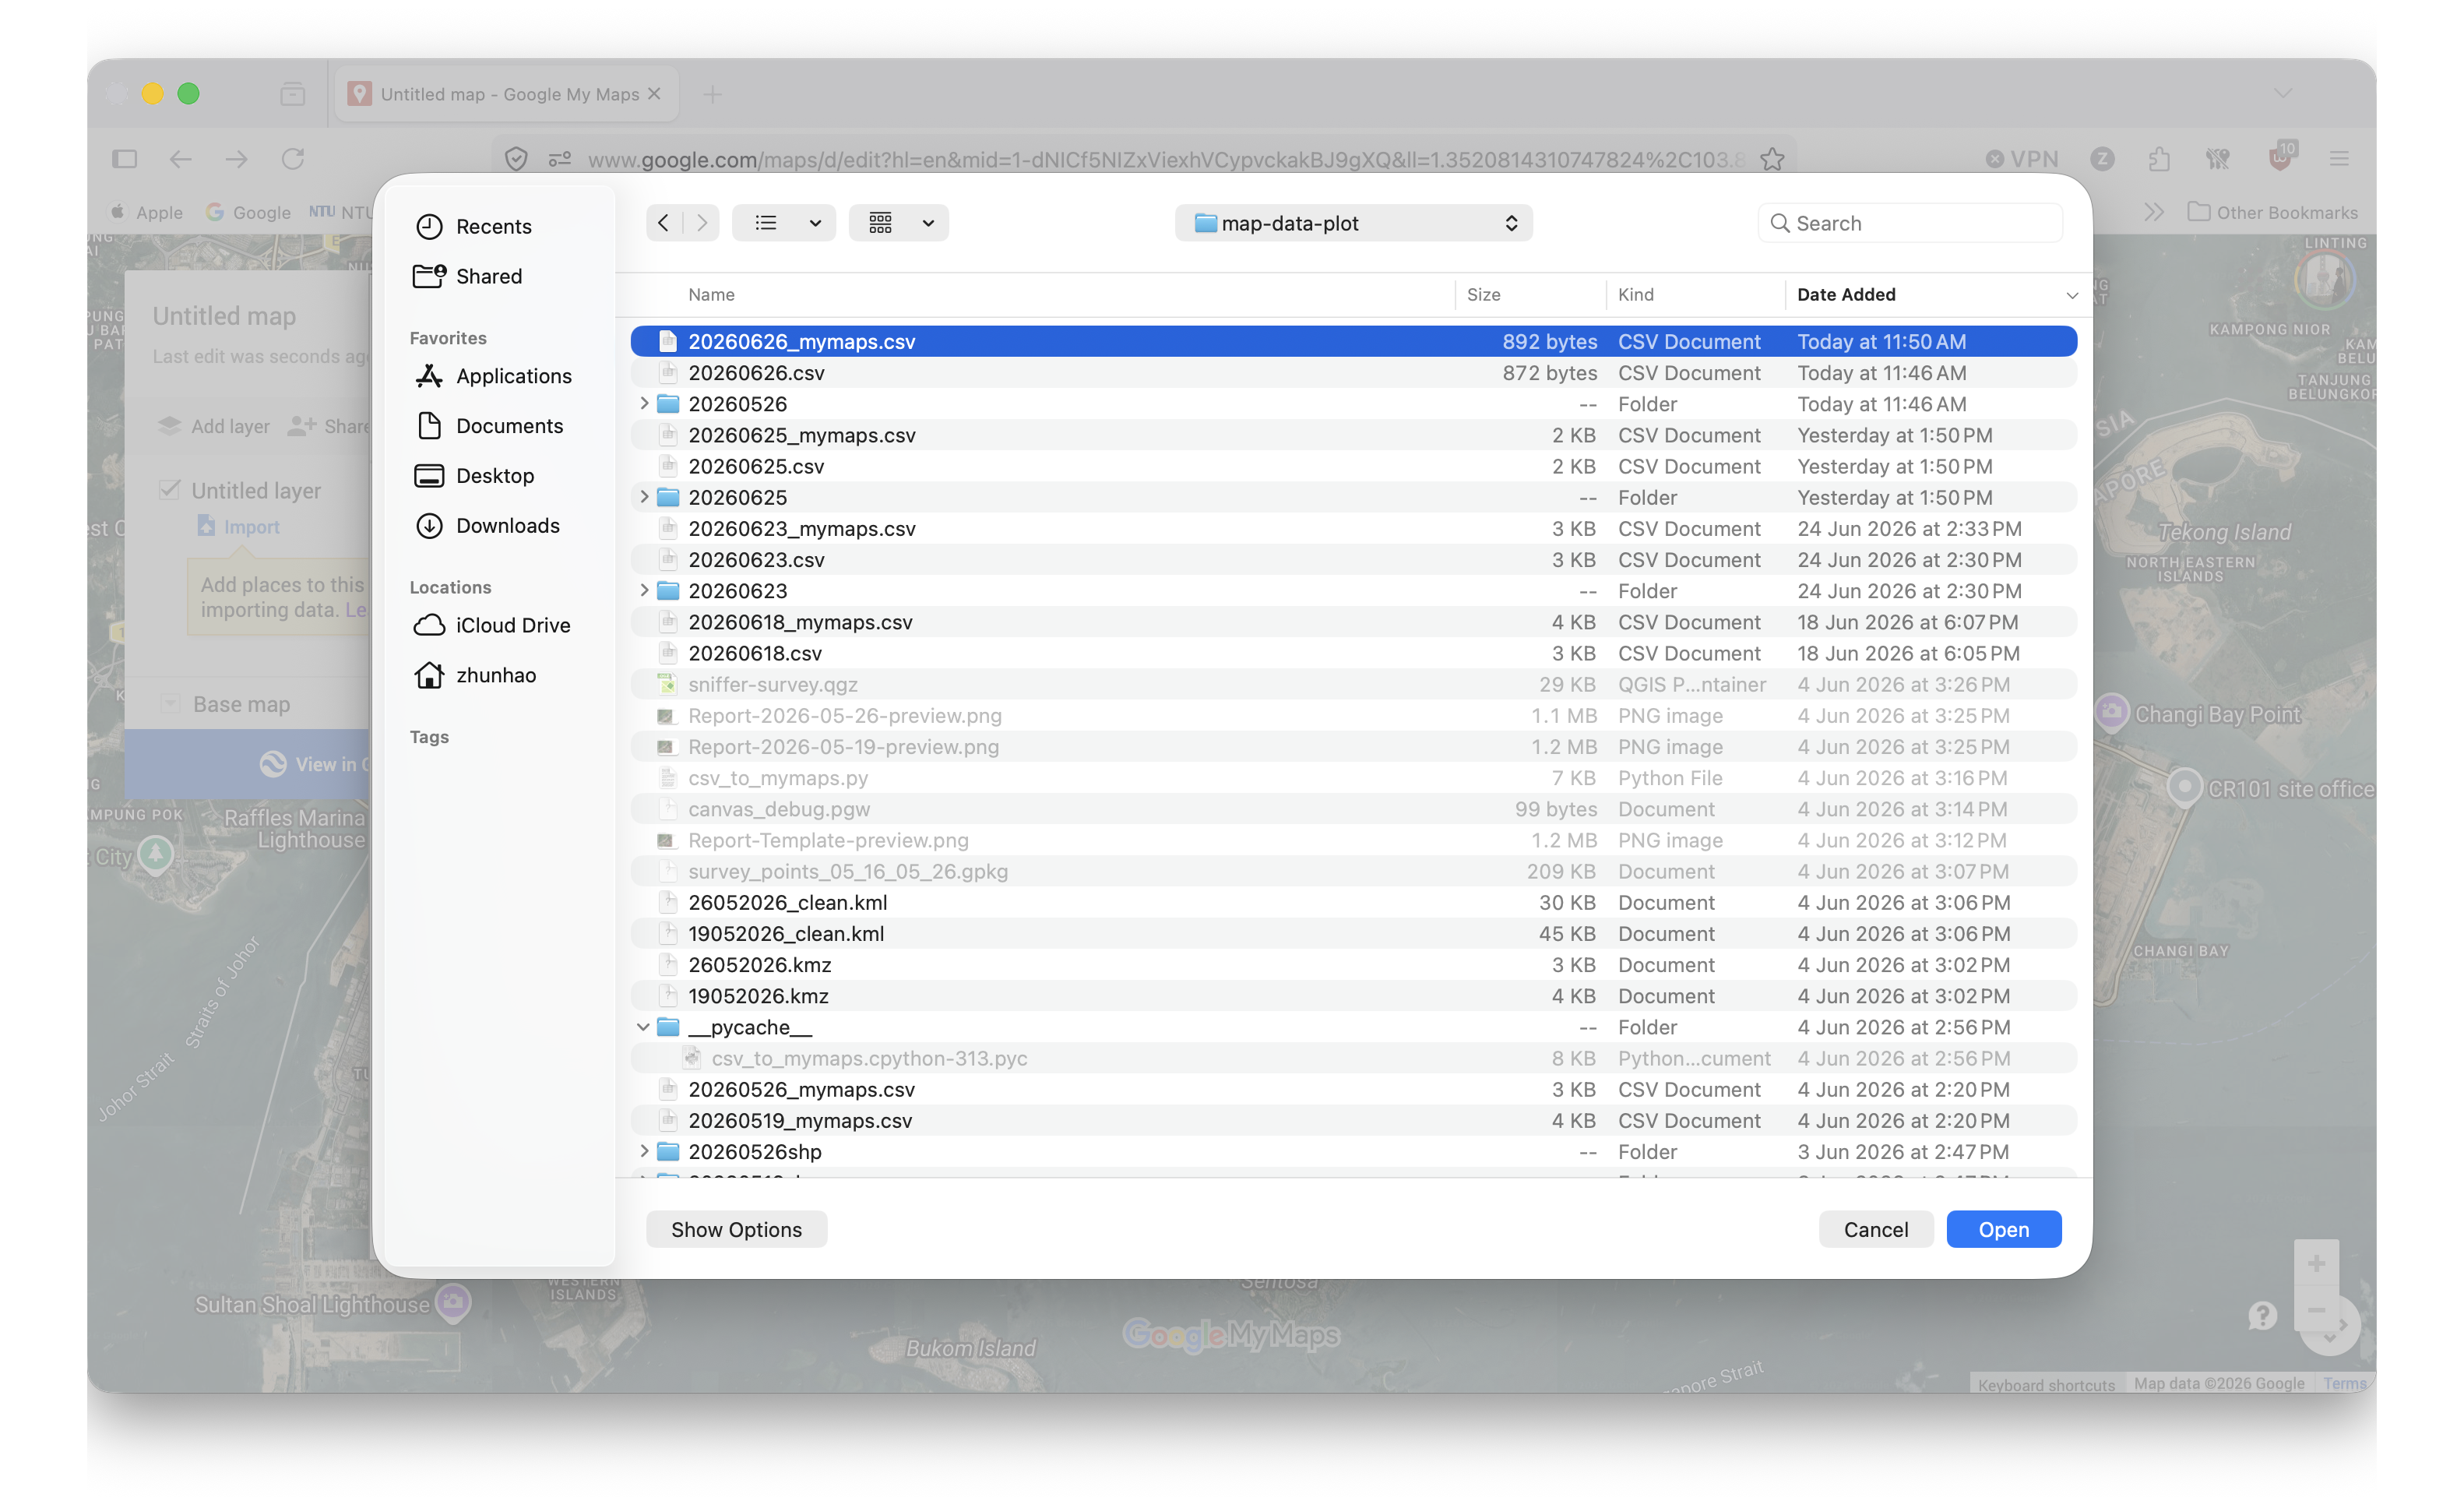
\includegraphics[width=1.0\textwidth]{images/pick_csv.png}
    \caption*{File browser picker showing selection of the translated 20260626\_mymaps.csv file.}
\end{figure}

\subsection{Step 26: Map Coordinates to Position Placemarks}
In the "Choose columns to position your placemarks" dialog box:
\begin{itemize}
    \item Check the boxes next to \textbf{Latitude} and \textbf{Longitude}.
    \item Confirm that these columns match their respective latitude and longitude coordinates.
    \item Click \textbf{Continue}.
\end{itemize}

\begin{figure}[H]
    \centering
    \includegraphics[width=0.8\textwidth]{images/screenshot_115358.png}
    \caption*{Mapping the Latitude and Longitude columns to position the survey marks.}
\end{figure}

\clearpage

\subsection{Step 27: Select Title for Markers}
In the "Choose a column to title your markers" dialog box:
\begin{itemize}
    \item Select the \textbf{Point Name} column.
    \item Click \textbf{Finish} to process and plot the data points.
\end{itemize}

\begin{figure}[H]
    \centering
    \includegraphics[width=0.8\textwidth]{images/screenshot_115404.png}
    \caption*{Choosing the Point Name column to act as labels for the markers.}
\end{figure}

\subsection{Step 28: Verify Plotted Survey Points}
The survey points (e.g. \texttt{Pt1}) are now successfully plotted on the map. Tapping any point reveals its full metadata, including Northing, Easting, elevation, time, antenna height, precision estimates (HRMS, VRMS), satellite status, and original/base coordinates.

\begin{figure}[H]
    \centering
    \includegraphics[width=1.0\textwidth]{images/screenshot_115412.png}
    \caption*{The final mapped points visualized with full satellite survey attribute readouts.}
\end{figure}

\end{document}
